\documentclass{cernatsnote}
\usepackage[colorinlistoftodos]{todonotes}
\usepackage{placeins}
\usepackage{pdflscape}
\usepackage[para,online,flushleft]{threeparttable}
\title{Sextupole scheme optimization for the HL-LHC}
\author{
	Fabien Plassard$^{\dagger}$, Riccardo De Maria, Massimo Giovannozzi \; \\		
	CERN, CH-1211 Geneva, Switzerland
}
\email{fabien.plassard@cern.ch}
\date{\today}

\begin{document}
\maketitle

\begin{abstract}
 The strong squeeze of the beta-functions at the interaction points hosting the high-luminosity experiments ATLAS (Point 1) and CMS (Point 5) is one essential upgrade of the High-Luminosity LHC project (HL-LHC) to reach the desired luminosity.
 In order to overcome various limitations imposed by the machine to reduce the beta-functions to very low values, the achromatic telescopic squeeze (ATS) approach has been adopted for the HL-LHC. The present implementation of the scheme foresees the installation of an additional sextupole in the lattice around Point 1 and Point 5 to increase dynamic aperture (DA). This report studies alternative implementations of the ATS scheme that could mitigate the absence of the sextupole in Q10 (named MS10).
 
 
 %The resulting large beta waves at the sextupole locations excite strong nonlinearities that are compensated in the baseline design by adding four additional sextupoles in the lattice. This allows to keep the long term survival of the beam, referred to as the dynamic aperture (DA), to a viable level for operation. In this study, alternative sextupole lattices are proposed. These lattices have the advantage of avoiding the costly and time consuming installation of the additional sextupoles, while keeping the DA at the required level and the optics parameters within the constraints. The optimization process and the impact on the linear optics, aberrations and dynamic apertures are summarized in this paper.

\end{abstract}
\\ \\ \\ 

\begingroup
\color{black}
\tableofcontents
\endgroup

\pagebreak

\section{Introduction}

The design upgrade towards the high luminosity LHC (HL-LHC) forsees to push the LHC beam and optics parameters~\cite{hllhc_tdr} to enable the machine to deliver an integrated luminosity of at least 250 fb$^{-1}$ per year in the two high luminosity collision points IP1 and IP5 hosting the detectors ATLAS and CMS, respectively. One essential upgrade to reach the desired HL-LHC performance is the reduction of the transverse beam spot size at the IP which requires to squeeze down $\beta^{*}$, at constant emittances. In order to overcome various limitations imposed by the LHC quadrupoles and sextupoles to reduce the $\beta$ functions to very low $\beta^{*}$, a novel squeeze approach named achromatic telescopic squeeze (ATS)~\cite{ats} has been adopted for the HL-LHC.\\

The reduction of the IP $\beta$ functions from the so called pre-squeeze $\beta^{*}$ of 50~cm towards the ultimate squeeze $\beta^{*}$ of 15~cm, for the round optics, is performed by varying the matching quadrupole strengths located in the insertion regions IR8/2 and IR4/6 adjacent to IP1 and IP5, respectively. The resulting $\beta$ beating waves in the sectors 45, 56, 81 and 12 contributes to the $\beta^{*}$ squeeze while keeping the quadrupole strengths of the high luminosity insertions constant and, thanks to a proper phasing in the arc cell, keeping stable chromaticity correction with the strength of the lattice sextupoles nearly constant. The increase of the peak transverse $\beta_{x,y}$ at the strong sextupoles in the arcs during the squeeze excites sextupolar geometrical resonant driving terms (RDT) that rise with ATS factor. If they are left uncompensated, these geometrical aberrations induce tune spread and can strongly degrade the long term survival of the beam. Within each arc adjacent to IP1 and IP5, the non-linear kick generated by the strong sextupoles can be compensated two-by-two when separated by a $\pi$ phase advance between them. Therefore, a self-compensation of the geometrical aberrations excited during the ATS can be obtained if the strong sextupole families contain an even number of magnets.\\

In the current LHC sextupole lattice, there are 9 and 11 strong sextupoles in the arc 81 and 45 (arc 12 and 56 for Beam 2), respectively. Consequently, the HL-LHC optics baseline envisage the installation of an additional sextupole, named MS10, at the quadrupole Q10 in the IR1 and IR5 insertions. The additional MS10 has a positive impact on the dynamic aperture (DA) and has also the advantage of reducing the excitation level required for the strong sextupoles. Section~\ref{ms10} first recalls the impact of this additional sextupoles on RDTs and DA. Alternative sextupole lattice and optics have been studied and can restore self-compensation of the non-linear resonances to the same level as the baseline optics without MS10. These lattices have the advantage of avoiding the time-consuming interventions for the installation of the 4 needed additional cryostats and sextupoles. The optics changes and performances of these alternative designs are discussed in Section~\ref{alternative} and follow the studies started in~\cite{slhcv3,ms10_ppt1,ms10_ppt2}. The final performances of the different proposed optics are discussed in Section~\ref{phase_optim15} where the phase advances between the two low-$\beta^{*}$ IPs are tuned in order to increase further the DA. The simulations shown in this report are based on the current latest version of the HL-LHC layout, HLLHCV1.4~\cite{hllhcv14}.


\section{MS10 sextupole for HL-LHC: aberrations and long term stability} \label{ms10}

The need of changes in the sextupole lattice from the LHC optics, to keep the machine DA at a viable level, has been proposed in past studies~\cite{ats,slhcv3,ms10_ppt1,ms10_ppt2}. Here, one presents a detailed quantitative comparison of the performances expected between the HL-LHC baseline optics and the LHC-like configuration which features an odd number of strong sextupoles in the arcs neighboring IR1 and IR5 insertions. Observations were performed on the non-linear resonances, tune footprints and long term stability of the beam.

\subsection{Sextupole lattice layout}

The strong sextupoles are located in sectors 81, 12, 45, 56 where the $\beta$-beating waves reach their maxima. They are responsible for the full correction of the natural chromaticity generated by the triplets and for half of the correction of the natural chromaticity generated by the quadrupoles located in the $\beta$-beating sectors. The remaining chromaticity is compensated by the local sextupole family. The LHC-like sextupole lattice, which is here referred to as the \textit{No MS10 optics}, features an odd number of focusing and defocusing strong sextupoles, as detailed in Table~\ref{tab_circuit_ms10}. For the current \textit{Baseline optics} of the HL-LHC, new focusing and defocusing strong sextupoles, named \textit{MS10F} and \textit{MS10D} respectively, will be installed at Q10. Figure~\ref{fig_twiss_base} shows the arrangement of the sextupoles and the $\beta_{x,y}$ functions in sectors 81 and 12 around IP1 (similar configuration for sectors 45 and 56 around IP5).The location of the new MS10F and MS10D for the Baseline optics are indicated in green in Fig~\ref{fig_twiss_base}.

\begin{table}
\begin{center}
\caption{\label{tab_circuit_ms10}  Sextupole circuits (in parenthesis the number of magnets) in Point 1 and Point 5 by category. Strong circuits are in phase with the triplet and used for chromatic corrections (chromaticity, off- momentum $\beta$-beating and dispersion) from the triplet as well as from the arc. Local circuits compensate only chromaticity generated in the arcs.}
\begin{tabular}{lcccc} \hline
No MS10 circuit  &  Baseline circuit  &   Sectors    &    Beam     &   Category  \\ \hline
SF1 (\textbf{9}) , SD2 (\textbf{12})  &  SF1 (\textbf{10}), SD2 (\textbf{12})  &   81, 45    &    B1     &   Strong  \\ 
SF1 (\textbf{10}), SD2 (\textbf{11})  &  SF1 (\textbf{10}), SD2 (\textbf{12})  &   12, 56    &    B1     &   Strong  \\ 
SF2 (\textbf{10}), SD1 (\textbf{11})  &  SF2 (\textbf{10}), SD1 (\textbf{12})  &   81, 45    &    B2     &   Strong  \\ 
SF2 (\textbf{9}) , SD1 (\textbf{12})  &  SF2 (\textbf{10}), SD1 (\textbf{12})  &   12, 56    &    B2     &   Strong  \\ 
SF2 (\textbf{10}), SD1 (\textbf{12})  &  SF2 (\textbf{10}), SD1 (\textbf{12})  &   81, 45    &    B1     &   Local  \\ 
SF2 (\textbf{10}), SD1 (\textbf{12})  &  SF2 (\textbf{10}), SD1 (\textbf{12})  &   12, 56    &    B1     &   Local  \\ 
SF1 (\textbf{10}), SD2 (\textbf{12})  &  SF1 (\textbf{10}), SD2 (\textbf{12})  &   81, 45    &    B2     &   Local  \\ 
SF1 (\textbf{10}), SD2 (\textbf{12})  &  SF1 (\textbf{10}), SD2 (\textbf{12})  &   12, 56    &    B2     &   Local  \\ \hline
\end{tabular}
\end{center}
\end{table}

\begin{figure}[h!]
\centering
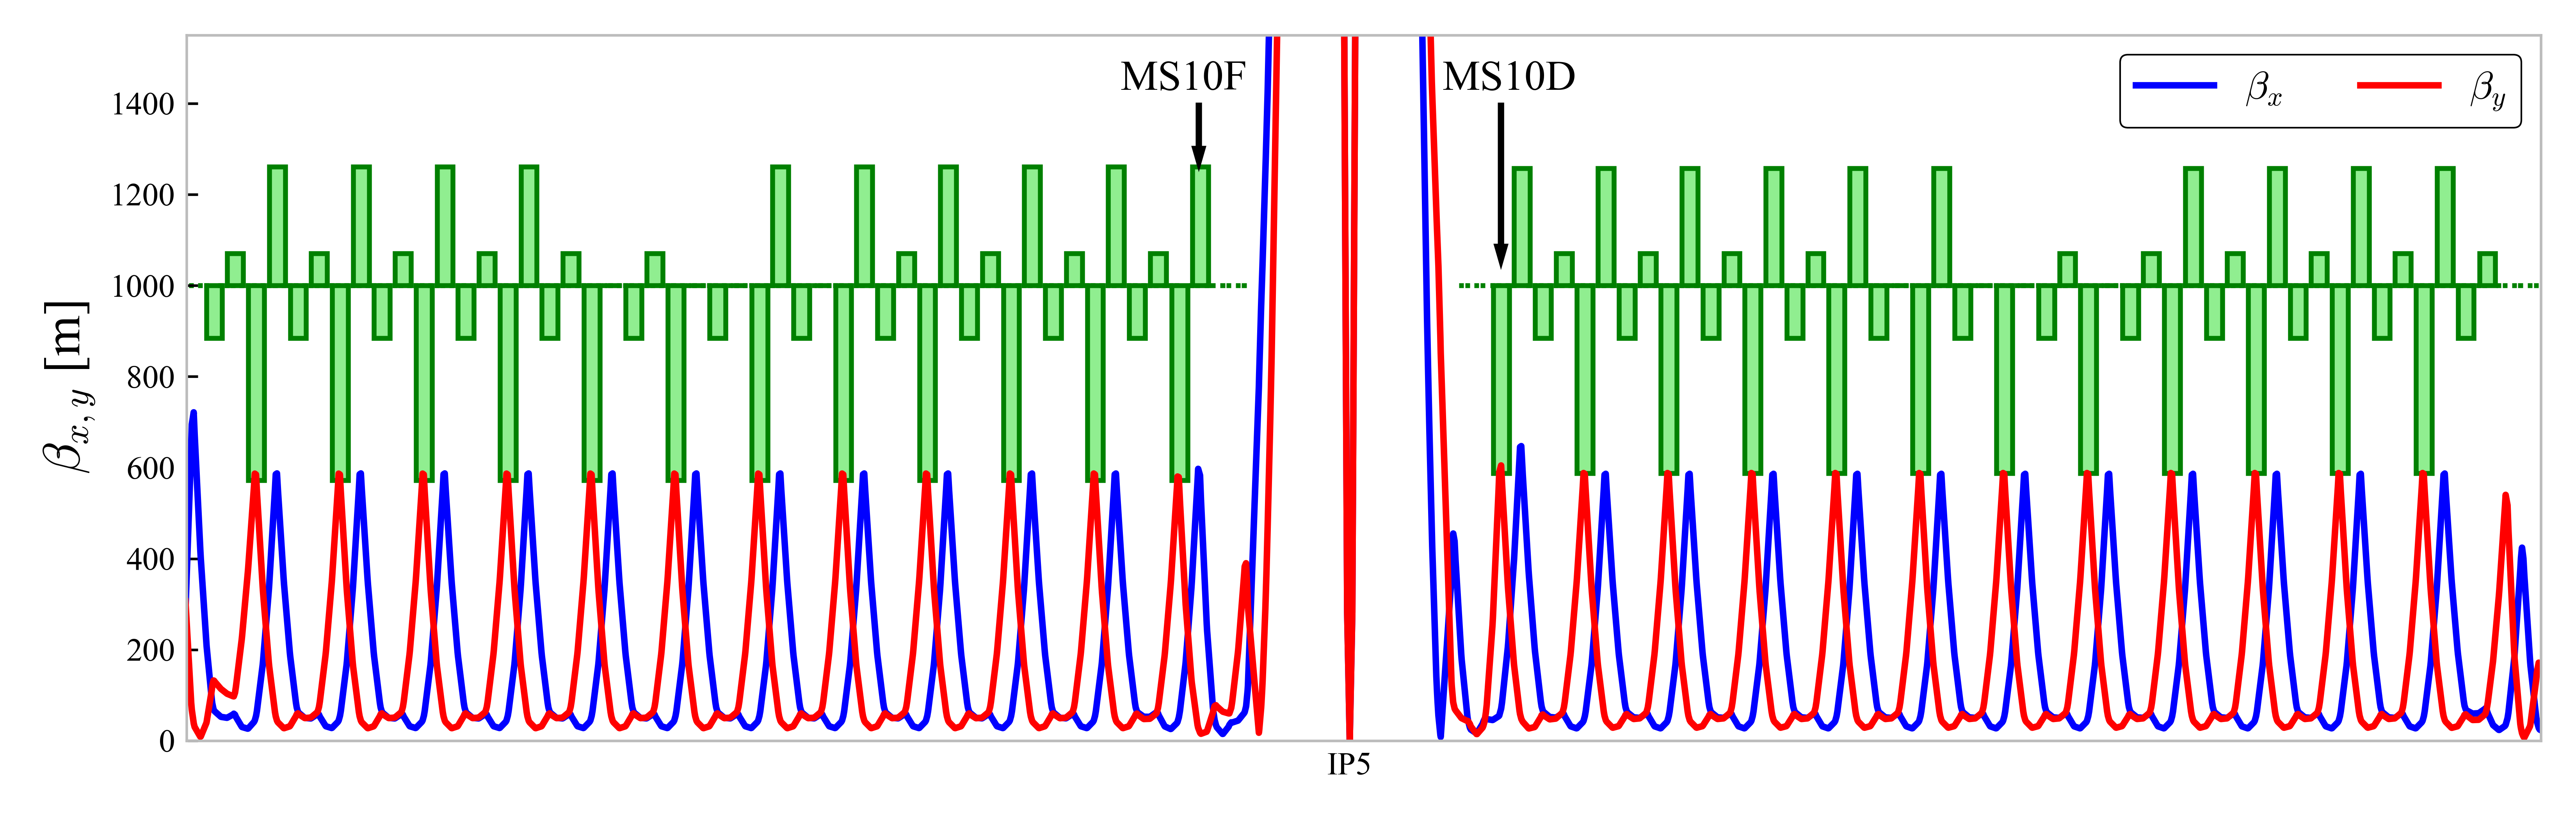
\includegraphics[width=1.0\textwidth]{images/lattice_sext_base.png}
\caption{\label{fig_twiss_base} Sextupole scheme (green lines) around IP5 of the Baseline optics for HL-LHC with the additional focusing and defocusing strong sextupoles MS10F and MS10D. The optics and sextupole scheme are similar around IP1.}
\end{figure}


\subsection{Geometrical Resonant Driving Terms and Footprint comparison}

The horizontal and vertical betatron phase advances are matched to $\Delta\mu_{x,y} = \pi$ between two consecutive focusing (or defocusing) strong sextupoles. Thanks to the designed $\pi$ phase advance, the equal strength and amplitudes $\beta_{x,y}$ within these pairs of sextupoles, one obtain a full two-by-two cancellation of the non-linear kicks generated by each strong sextupole. If one strong sextupole is not paired (odd number of magnets), as for the No MS10 optics, its uncompensated sextupole field will propagate through the ring. Figure~\ref{rdt_twiss_ms10} shows the cumulative sum as function of $s$ of the main sextupolar geometrical aberrations for the Baseline and No MS10 optics at $\beta_{x,y}^{*}$~=~15~cm.
\begin{figure}[h!]
\centering
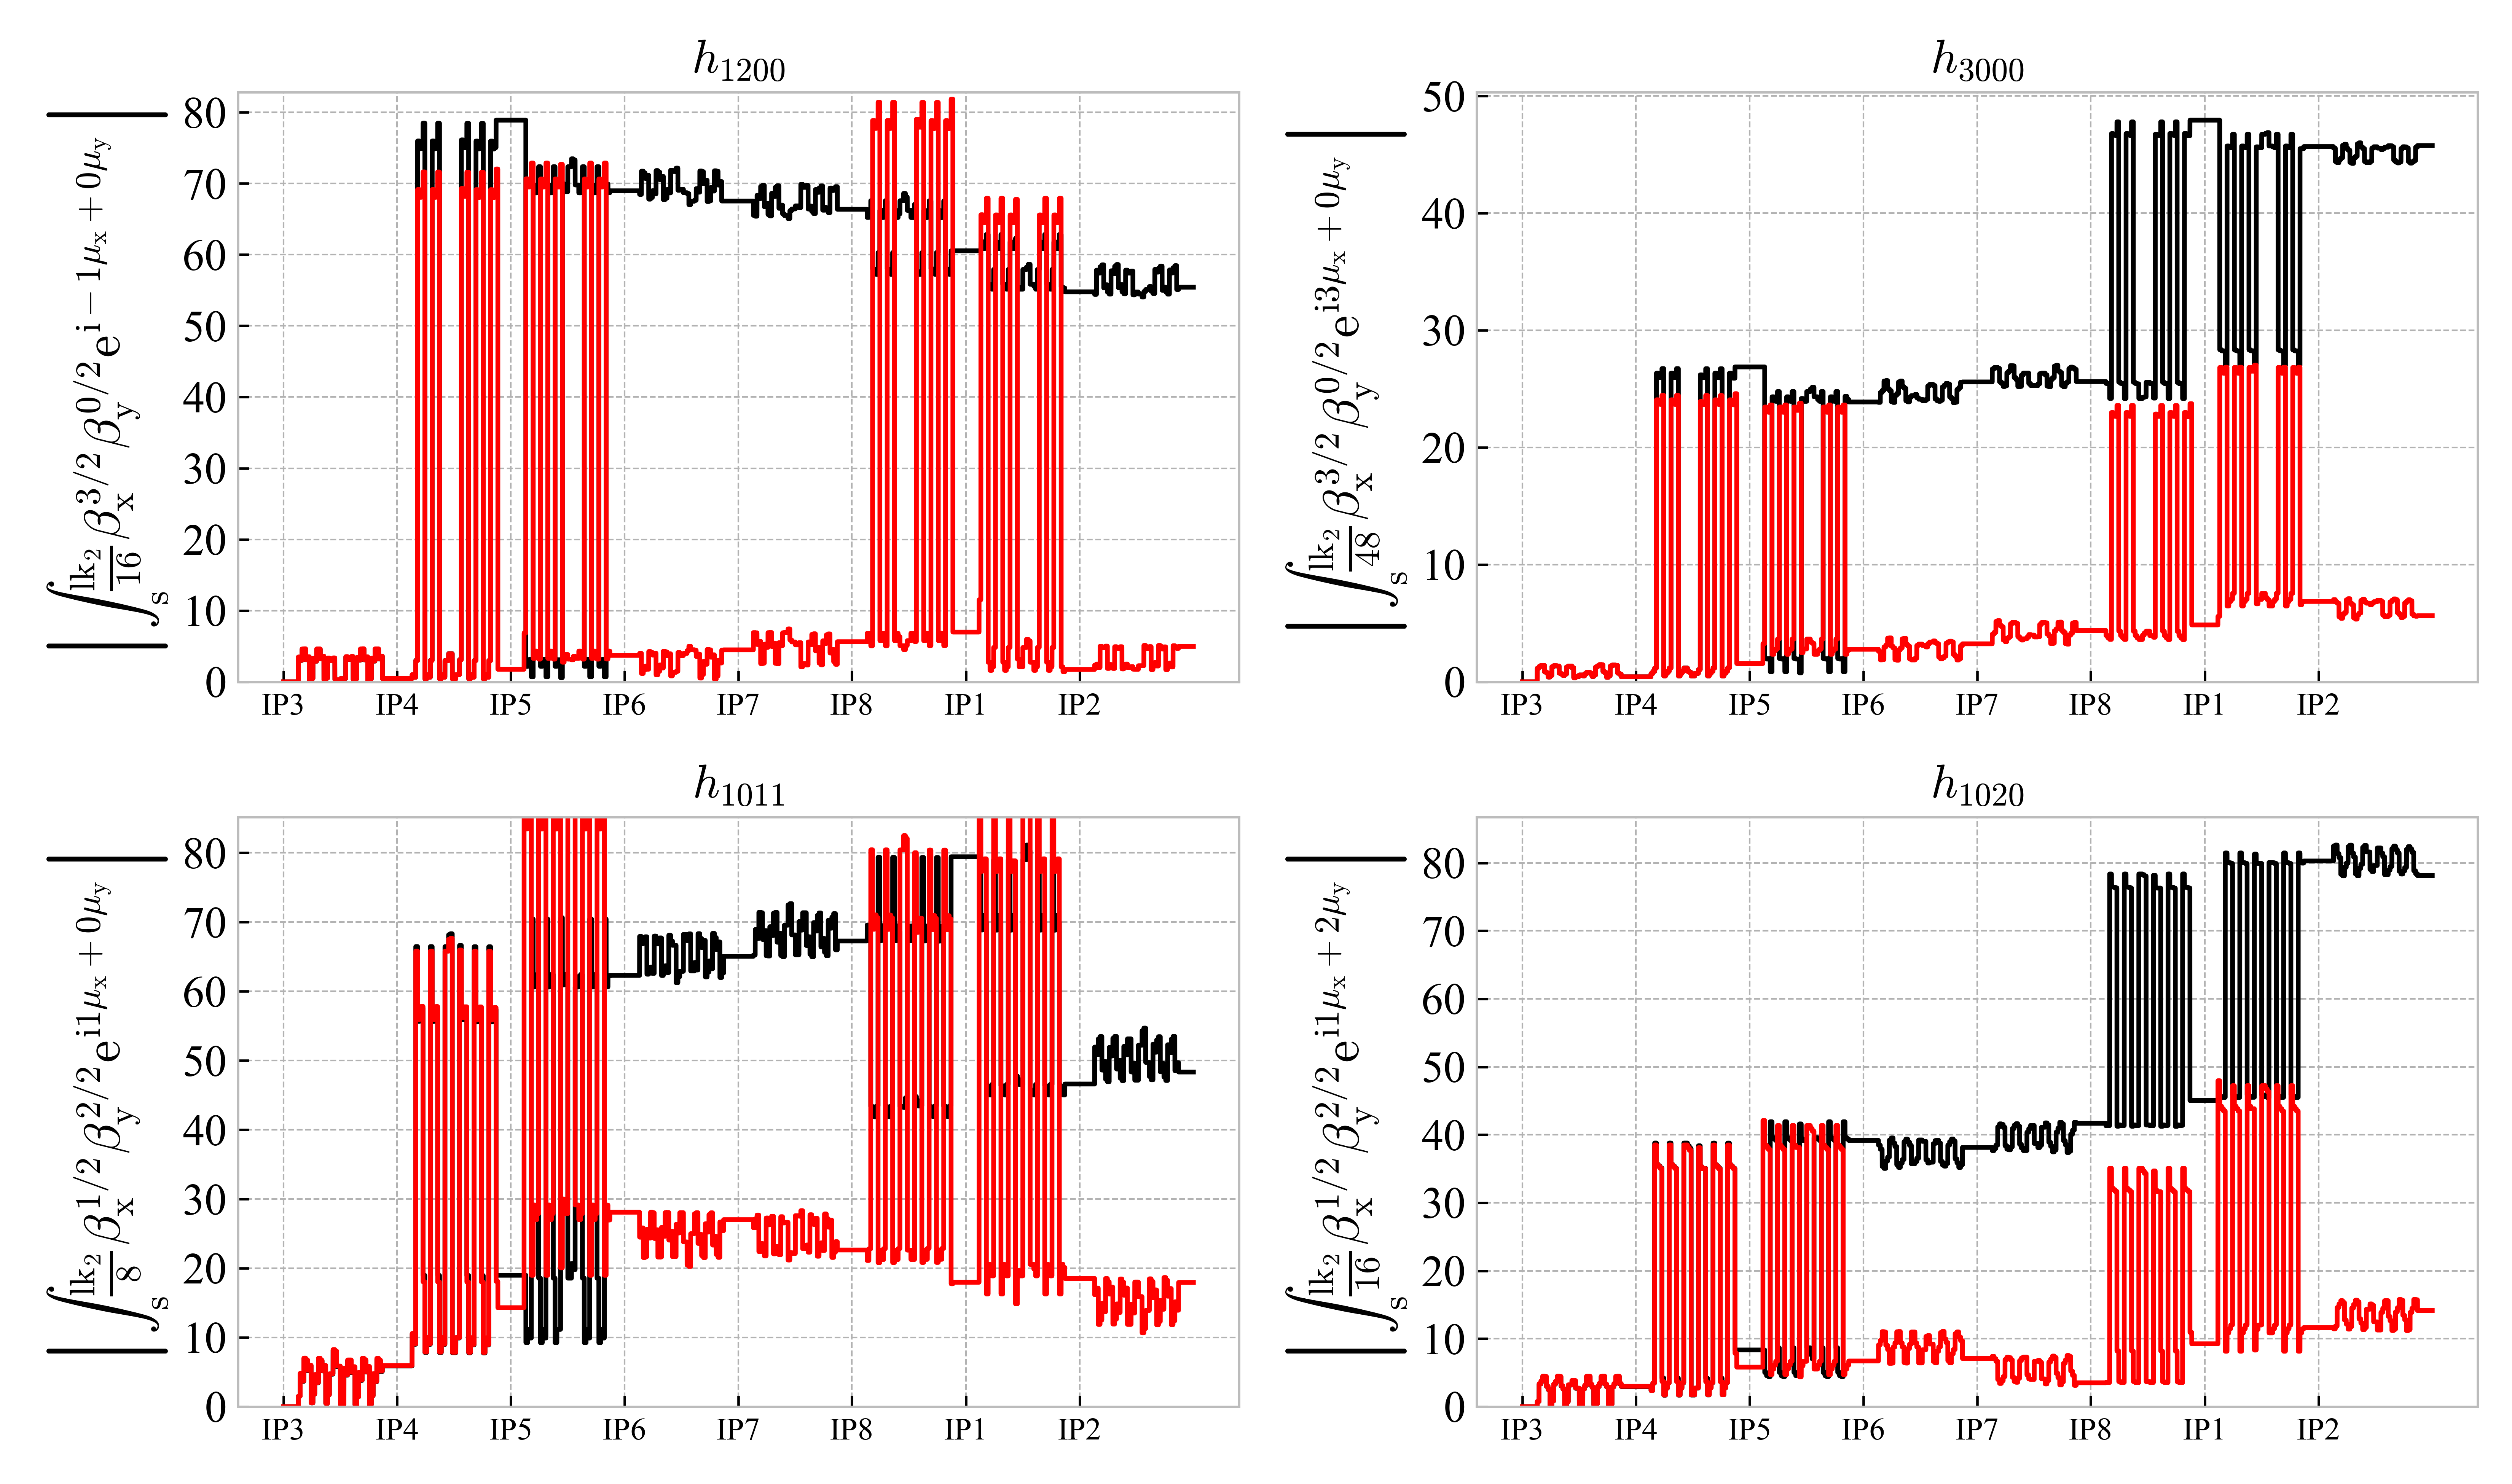
\includegraphics[width=1\textwidth]{images/rdt_twiss_base.png}
%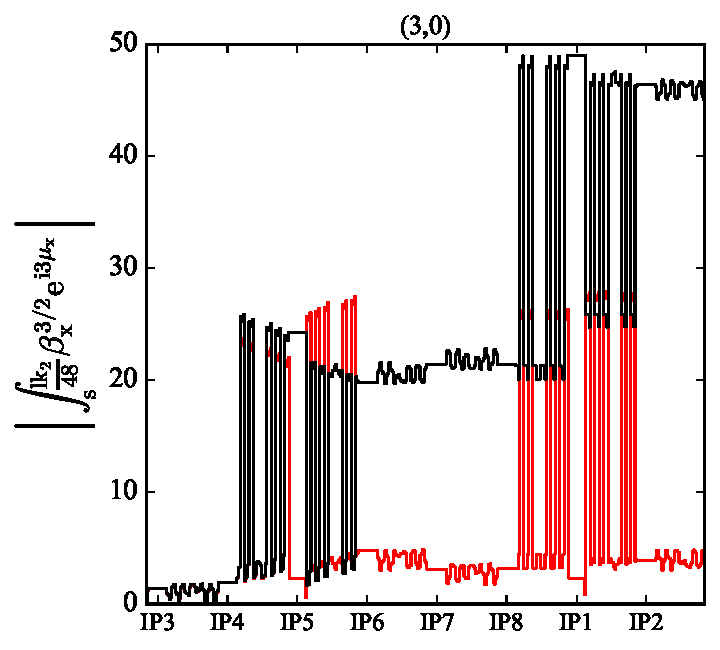
\includegraphics[width=0.49\textwidth]{images/3000_rdt_ms10_b1.pdf} \hfill 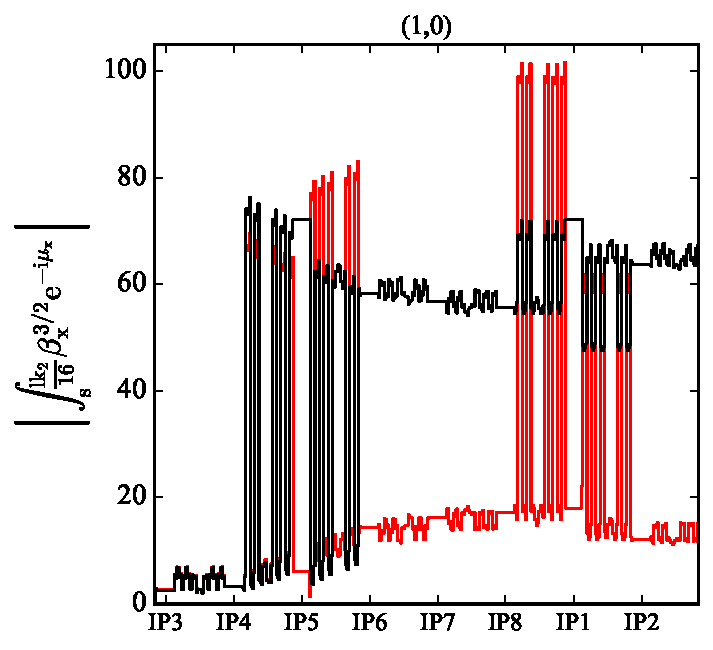
\includegraphics[width=0.49\textwidth]{images/1200_rdt_ms10_b1.pdf} \\
%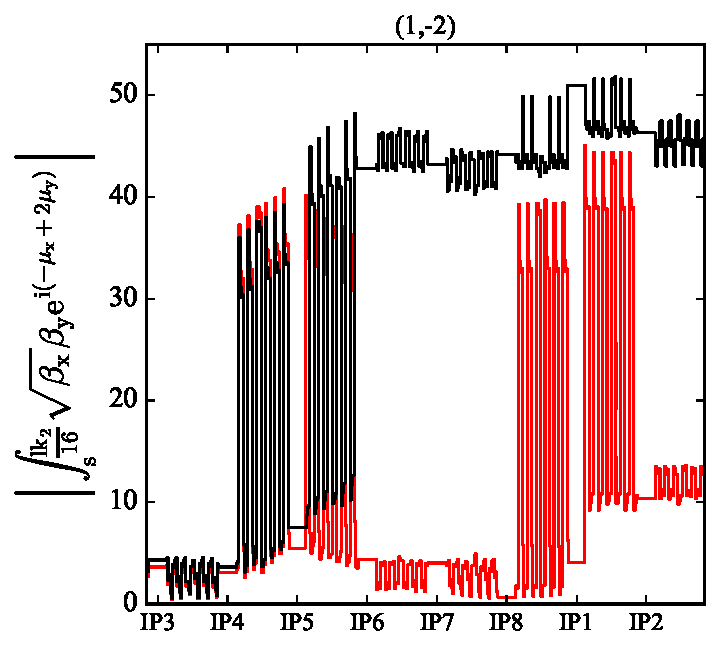
\includegraphics[width=0.49\textwidth]{images/0120_rdt_ms10_b1.pdf} \hfill 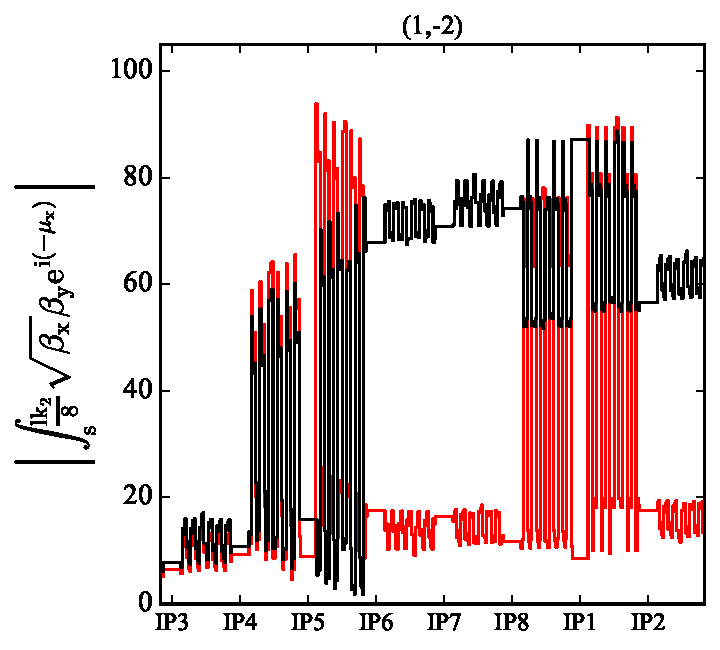
\includegraphics[width=0.49\textwidth]{images/0111_rdt_ms10_b1.pdf}
\caption{\label{rdt_twiss_ms10} Sextupole geometrical RDTs built-up along the ring with (Baseline optics) and without additional MS10.}
\end{figure}

\noindent The amplitude built-up of the normal geometrical resonant driving terms generated by the sextupole were computed from the Twiss functions using Eq.~\ref{eq_rdt},
\begin{equation}
\label{eq_rdt}
h_{jklm} = \frac{1}{j!k!l!m!2^{j+k+l+m}}\sum_{w} \mathrm{K}_{3,w} \beta_{x,w}^{\frac{j+k}{2}}\beta_{y,w}^{\frac{l+m}{2}}e^{i[(j-k)\Delta\mu_{x}+(l-m)\Delta\mu_{y}]} ,
\end{equation}

\noindent where $\mathrm{K}_{3,w}$ is the normal sextupole integrated strength at location index $w$. The contribution of the multipoles is of the order $n = 3 = j+k+l+m$, giving rise to terms in the Hamiltonian $\propto x^{j+k}y^{l+m}$. It is clear that restoring the pairs in the chain of the strong sextupoles allows a good control of these RDTs along the ring, which are enhanced with the ATS factor (ratio between the presqueeze $\beta^{*}$ and the squeeze $\beta^{*}$). The average amplitude of the normal and skew terms of order $n~=~3$ over the HL-LHC lattice for both optics and both Beam 1 (the clockwise beam) and Beam 2 (the counter-clockwise beam), were computed with PTC~\cite{ptc,twissrdt}. Figure~\ref{rdt_ptc_twiss_ms10} shows the different sextupolar RDTs for both beams using the crossing scheme at all IPs, as defined in~\cite{hllhc_param1,hllhc_param2}, with the orbit bumps of the dispersion correction and compares the situation for the Landau octupoles turned off and switched to their maximum strength of $k_{\mathrm{MO}}~=$~-570~A. In all cases, the normal terms of the geometrical aberrations are significantly larger in the case of the No MS10 optics compared with the one with the additional sextupole. These uncorrected aberrations have a sizeable impact on the footprint and leads to a significant increase of the level of tune diffusion in the case without MS10 as shown in Fig.~\ref{fma_ms10}. 

\begin{figure}[h!]
\centering
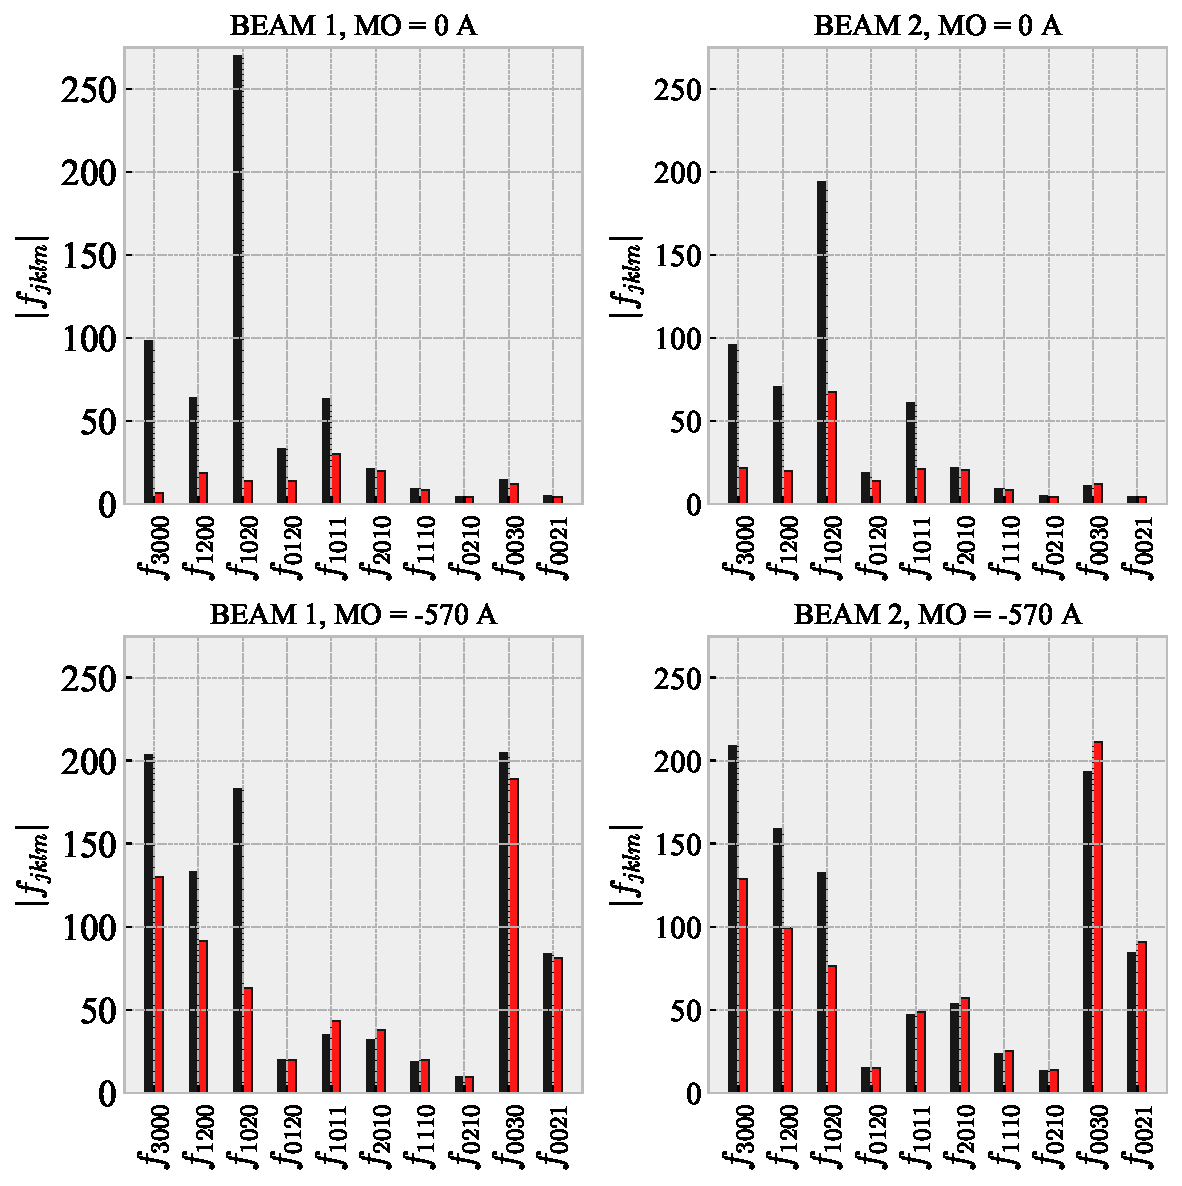
\includegraphics[width=0.9\textwidth]{images/rdt_sext_noms10_b12_oct_ca.pdf}
%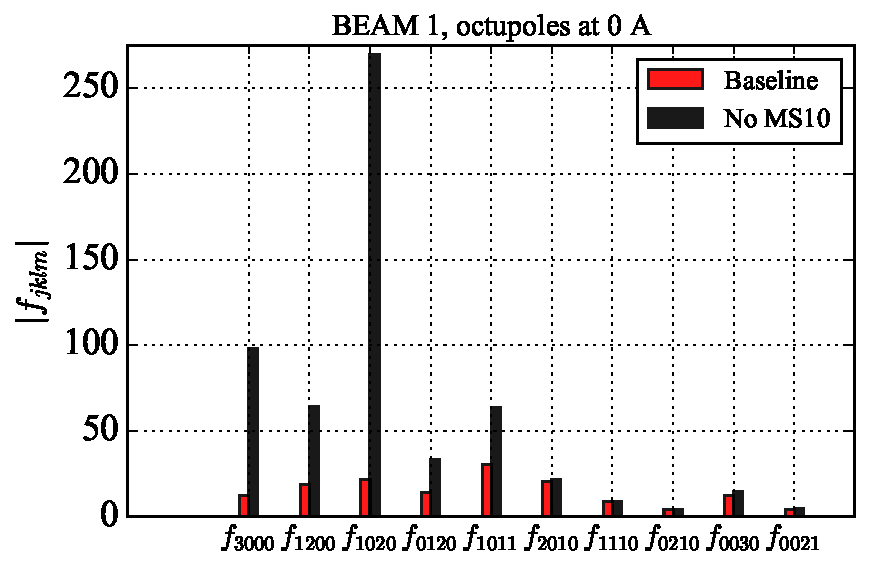
\includegraphics[width=0.49\textwidth]{images/rdt_sext_noms10_b1_0_ca.pdf} \hfill 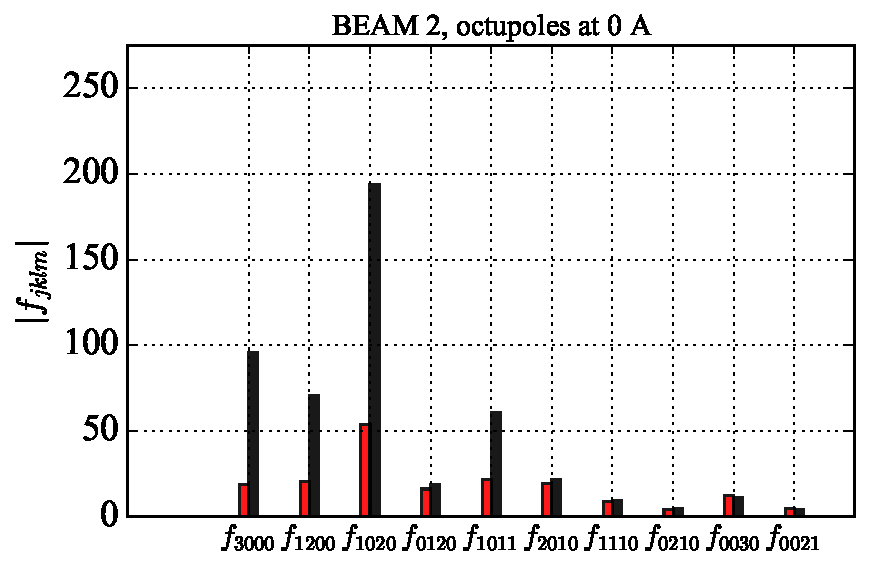
\includegraphics[width=0.49\textwidth]{images/rdt_sext_noms10_b2_0_ca.pdf} \\
%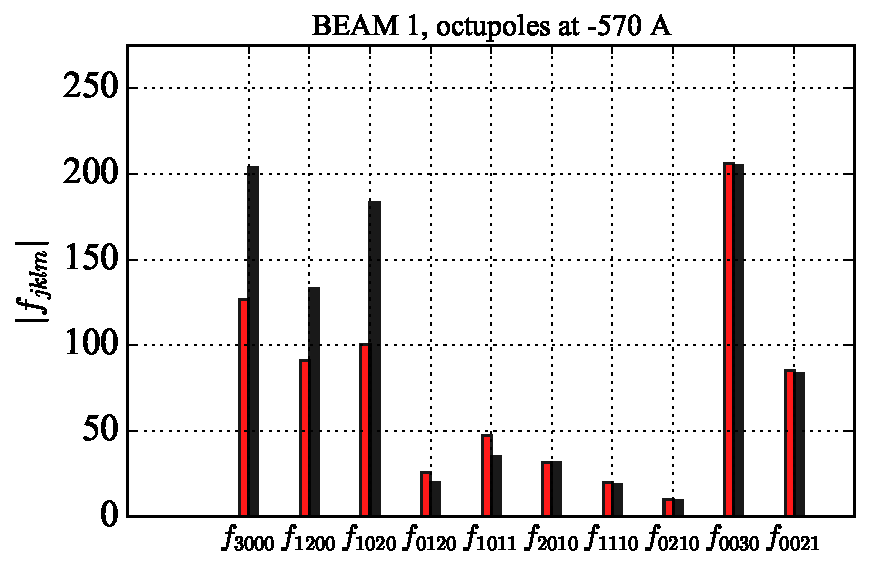
\includegraphics[width=0.49\textwidth]{images/rdt_sext_noms10_b1_570_ca.pdf} \hfill 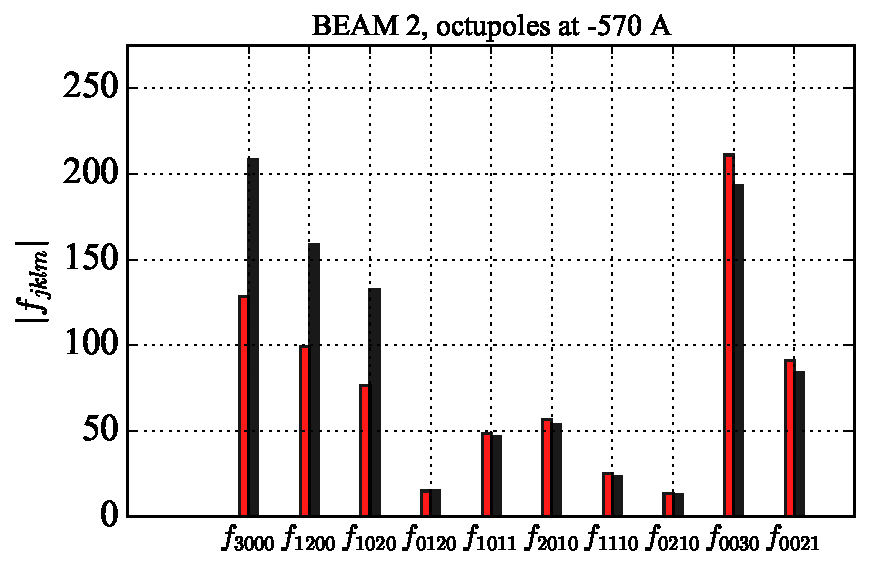
\includegraphics[width=0.49\textwidth]{images/rdt_sext_noms10_b2_570_ca.pdf}
\caption{\label{rdt_ptc_twiss_ms10} Average amplitude of the sextupole RDTs along the ring computed with PTC without (top plots) and with (bottom plots) Landau octupoles.}
\end{figure}

\begin{figure}[h!]
\centering
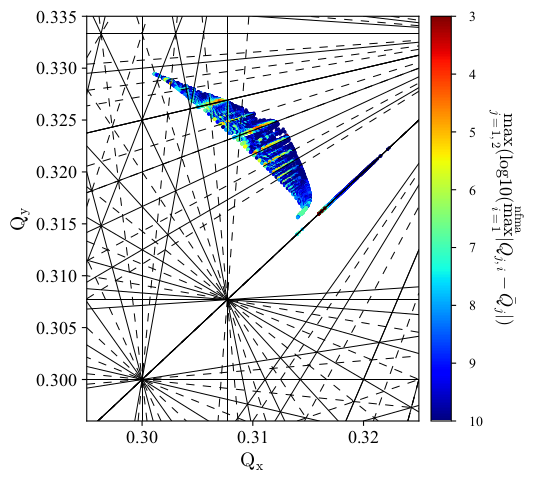
\includegraphics[width=0.49\textwidth]{images/fma_baseb1.png} \hfill 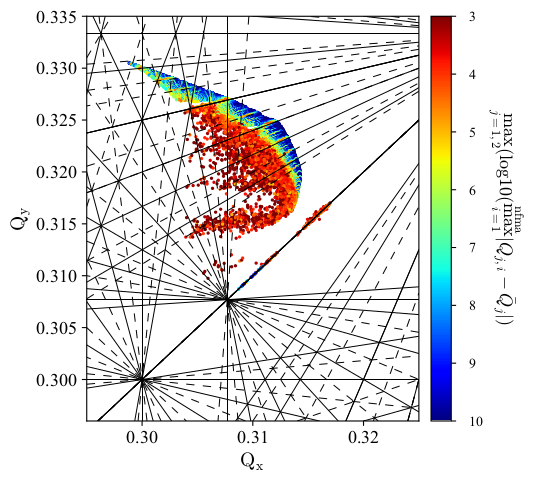
\includegraphics[width=0.49\textwidth]{images/fma_noms10b1.png} \\
\caption{\label{fma_ms10} Frequency Map Analysis on Beam 1 for the Baseline optics (left plot) and the No MS10 optics (right plot). Simulations performed at 10$\sigma$, $\delta_{p}$~=~2.7$\times 10^{-4}$,  $k_{\mathrm{MO}}~=$~-570~A, crossing scheme at all IPs defined in~\cite{hllhc_param1,hllhc_param2} and dispersion correction.}
\end{figure}

\subsection{Impact on DA}

The dynamic aperture was simulated using the tracking code SixTrack~\cite{six1,six2} and its running environment SixDesk~\cite{sixdesk}. The DA results are compared here between the LHC-like sextupole lattice and the Baseline optics for HL-LHC. The tracking conditions assumed for the simulations are as follow:\\
\begin{itemize}
    \item HLLHCV1.4 optics version at collision energy of 7~TeV with round optics and $\beta_{x,y}^{*}$~=~15~cm
    \item Tunes $Q_{x}$~=~62.31 and $Q_{y}$~=~60.32
    \item 30 particle pairs per 2$\sigma$ amplitude step tracked over 10$^{5}$ turns
    \item 5 $x-y$ phase-space angles
    \item chromaticity of 15 units and an energy spread $\delta p/p$ of 2.7$\times10^{-4}$
    \item normalized emittance $\epsilon_{n}$~=~2.5$\mu$m 
    \item half crossing angle $\theta/2$ at IP1/2/5/8 of 295/170/295/-250 $\mu$rad
    \item half parallel separation at IP1/2/5/8 of 0.75/2/0.75/-2 
    \item Landau octupole strengths $k_{\mathrm{MO}}$~=~-570~A (maximum strength)
    \item No Beam-Beam effects.
    \item 60 random error seeds for the generation of magnetic field errors
\end{itemize}

\noindent These simulation conditions, unless stated otherwise, are conserved for all DA results on the different optics options presented throughout this report. The impact on DA of the correction of the geometrical aberrations provided by the MS10 is large even on an error-free machine. Figure~\ref{da_ms10} shows the DA results considering operational conditions but without taking into account any non-linear field error in the HL-LHC magnets. Here, the \textit{average DA} or the \textit{minimum DA} is the average or minimum over the 59 phase-space angles (and over all seeds when imperfections are applied). In the LHC-like sextupole configuration, Beam 1 and 2 show an average DA of 8.7$\sigma$ and 9.5$\sigma$, respectively, compared to 12$\sigma$ and 11$\sigma$ with the additional MS10.

\begin{figure}[h!]
\centering
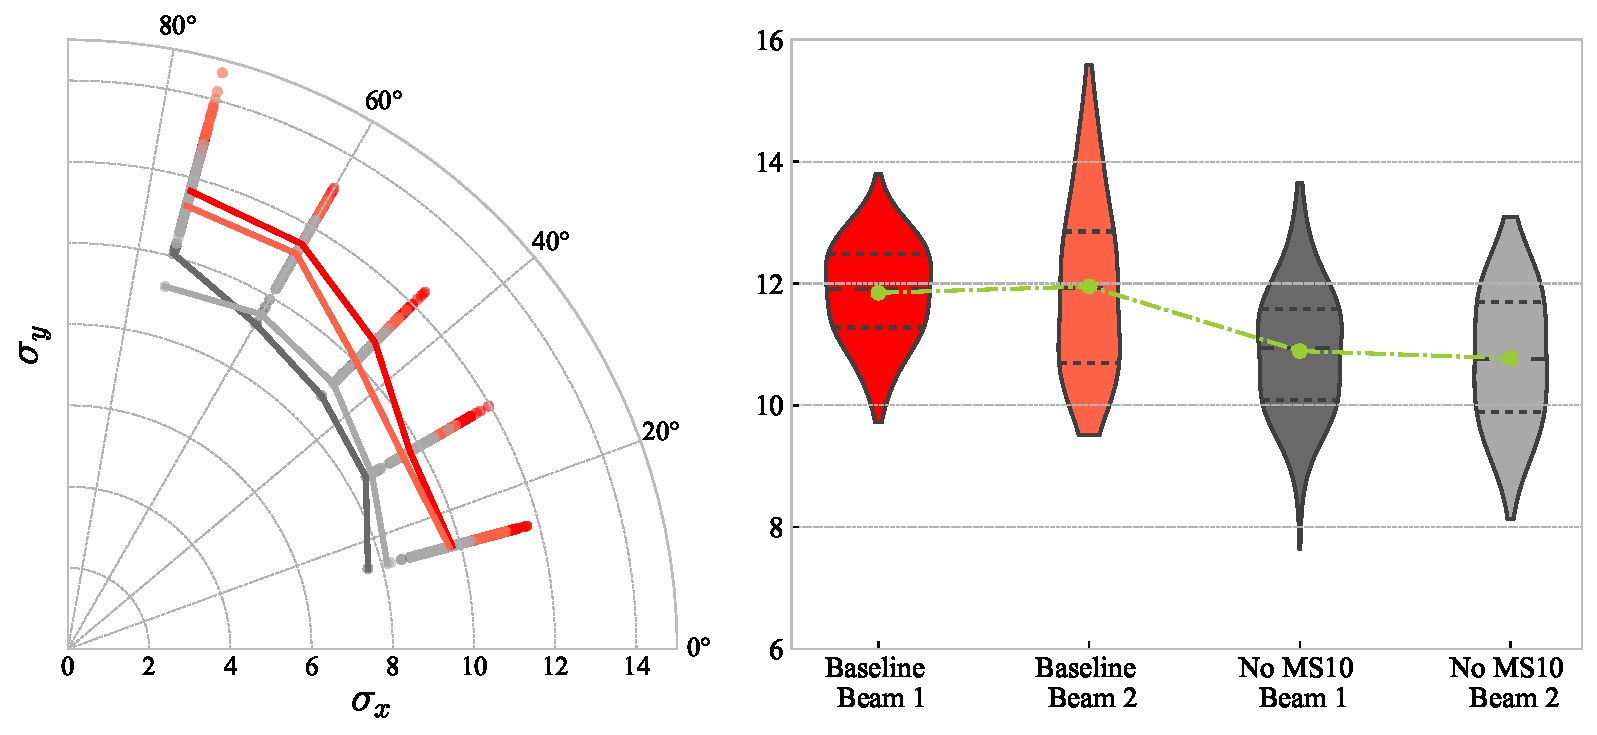
\includegraphics[width=1\textwidth]{images/da_imp_noms10.pdf}
\caption{\label{da_ms10} Dynamic aperture comparison between the Baseline and the No MS10 optics. The DA is simulated without multipolar imperfections, with crossing angle, dispersion correction and Landau octupoles set to their maximum strength of -570 A, after 10$^{6}$ turns and calculated over 59 angles. }
\end{figure}

\clearpage


\subsection{Phase optimization between IP1 and IP5 with MS10}

The phase between IP1 and IP5 has an important repercussion on the compensation of some fourth and higher order resonant driving terms and on the tune diagram which can results in visible degradation or improvement of the long term stability of the beam.   

%\begin{figure}[h!]
%\centering
%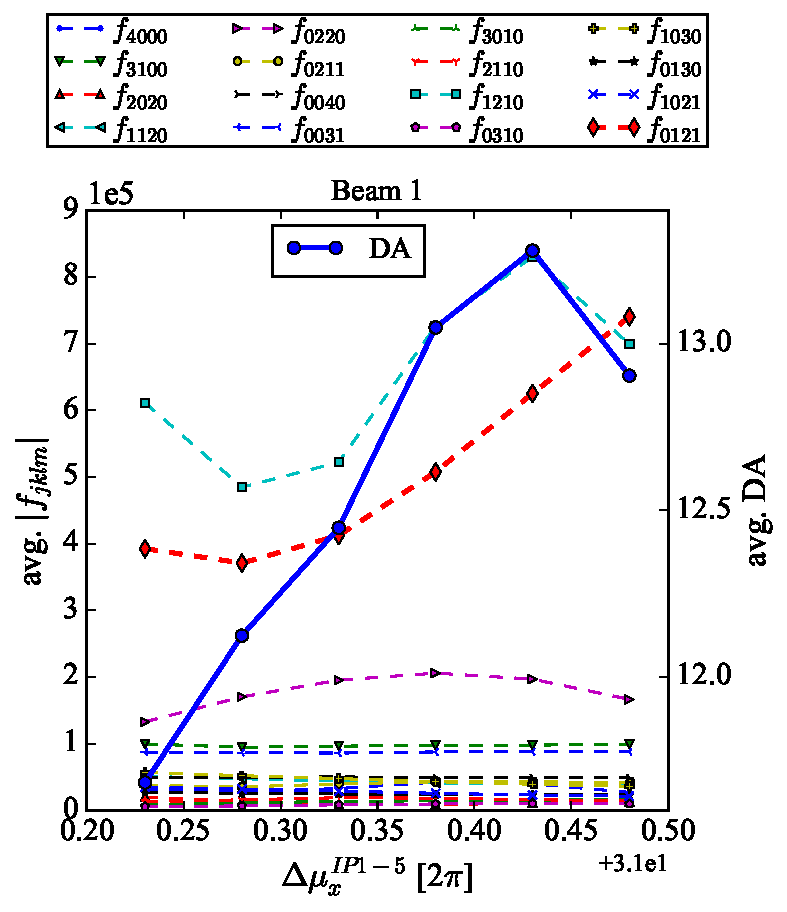
\includegraphics[width=0.49\textwidth]{images/rdt4_vs_phase_xbaseb1.pdf} \hfill 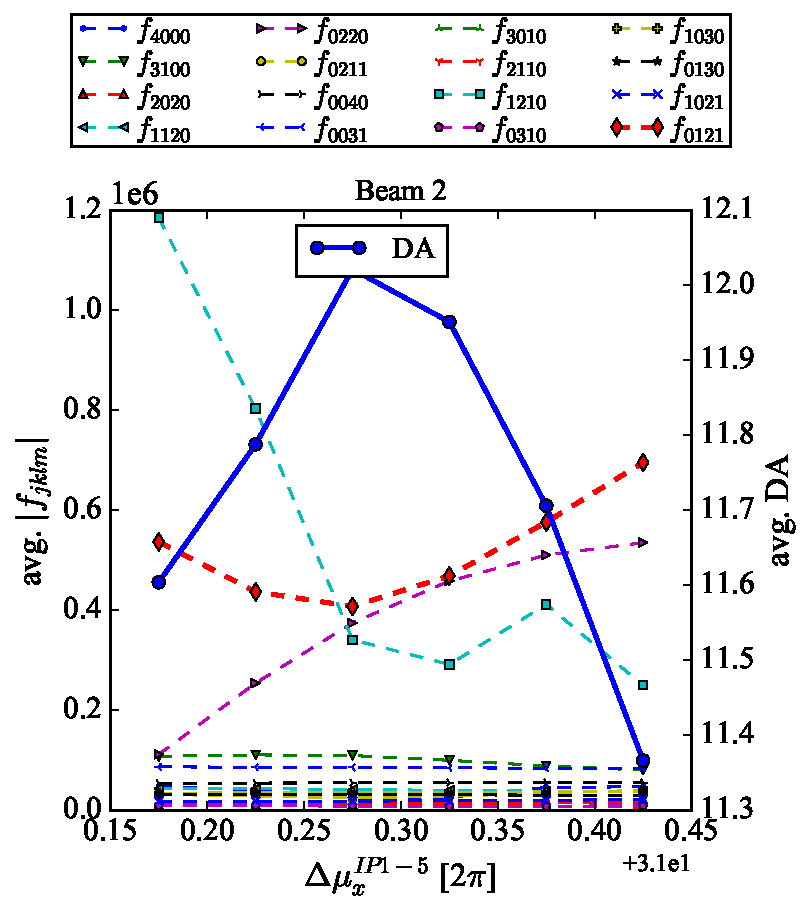
\includegraphics[width=0.49\textwidth]{images/rdt4_vs_phase_xbaseb2.pdf} \\
%\caption{\label{scan_da_vs_rdt_base_x} }
%\end{figure}

\begin{figure}[h!]
\centering
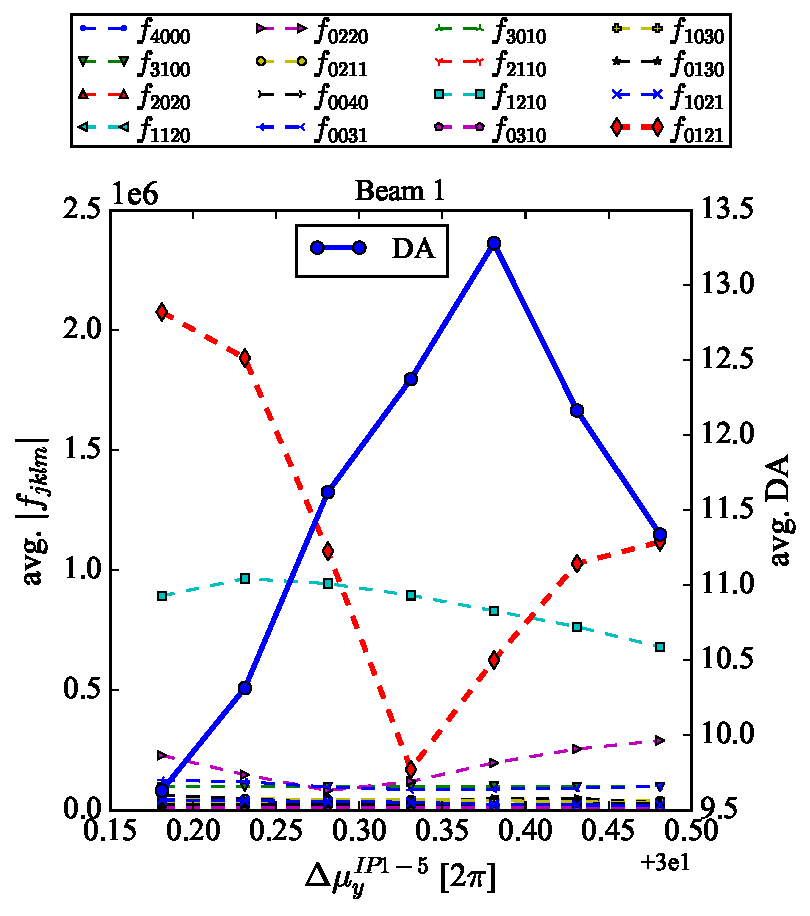
\includegraphics[width=0.49\textwidth]{images/rdt4_vs_phase_baseb1.pdf} \hfill 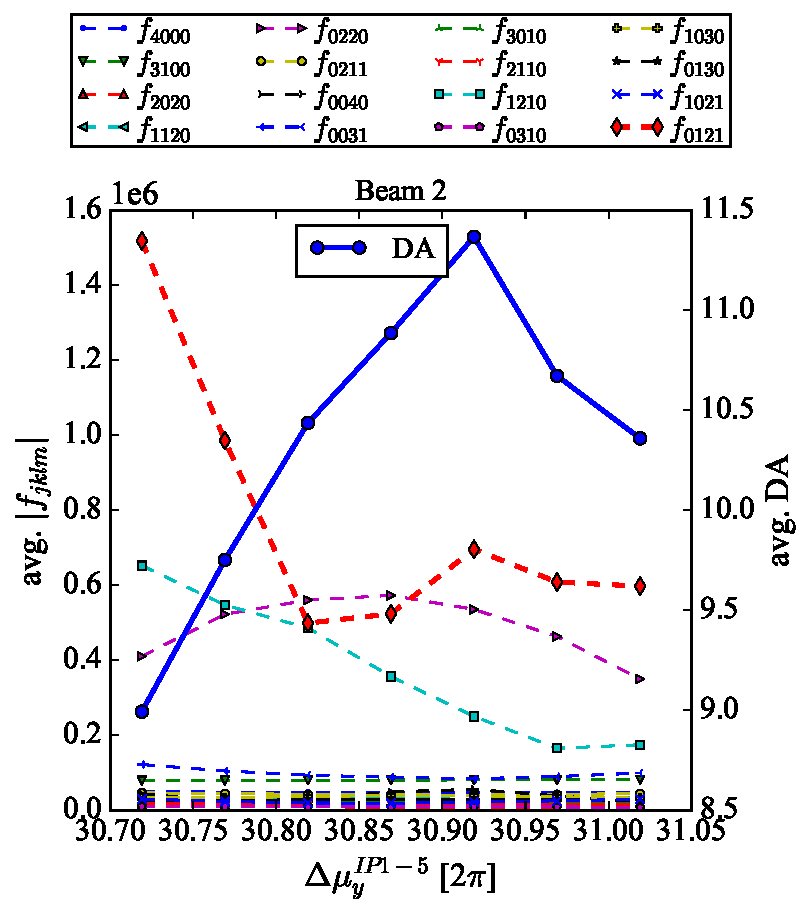
\includegraphics[width=0.49\textwidth]{images/rdt4_vs_phase_baseb2.pdf} \\
\caption{\label{scan_da_vs_rdt_base_x} }
\end{figure}


\begin{figure}[h!]
\centering
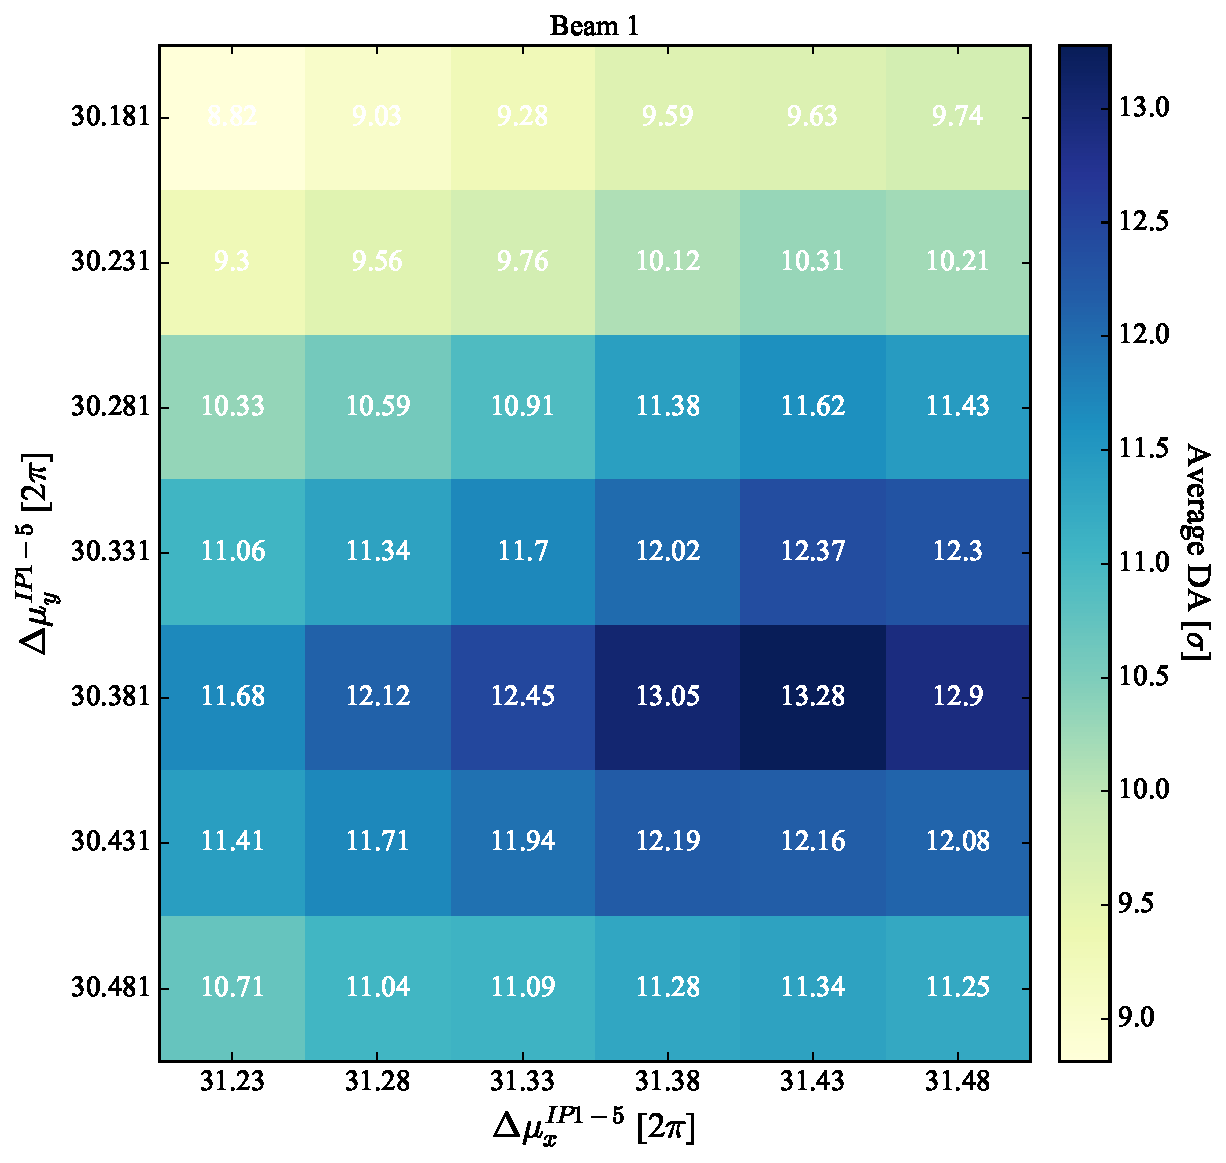
\includegraphics[width=0.49\textwidth]{images/scan_baseline_avg_b1.pdf} \hfill 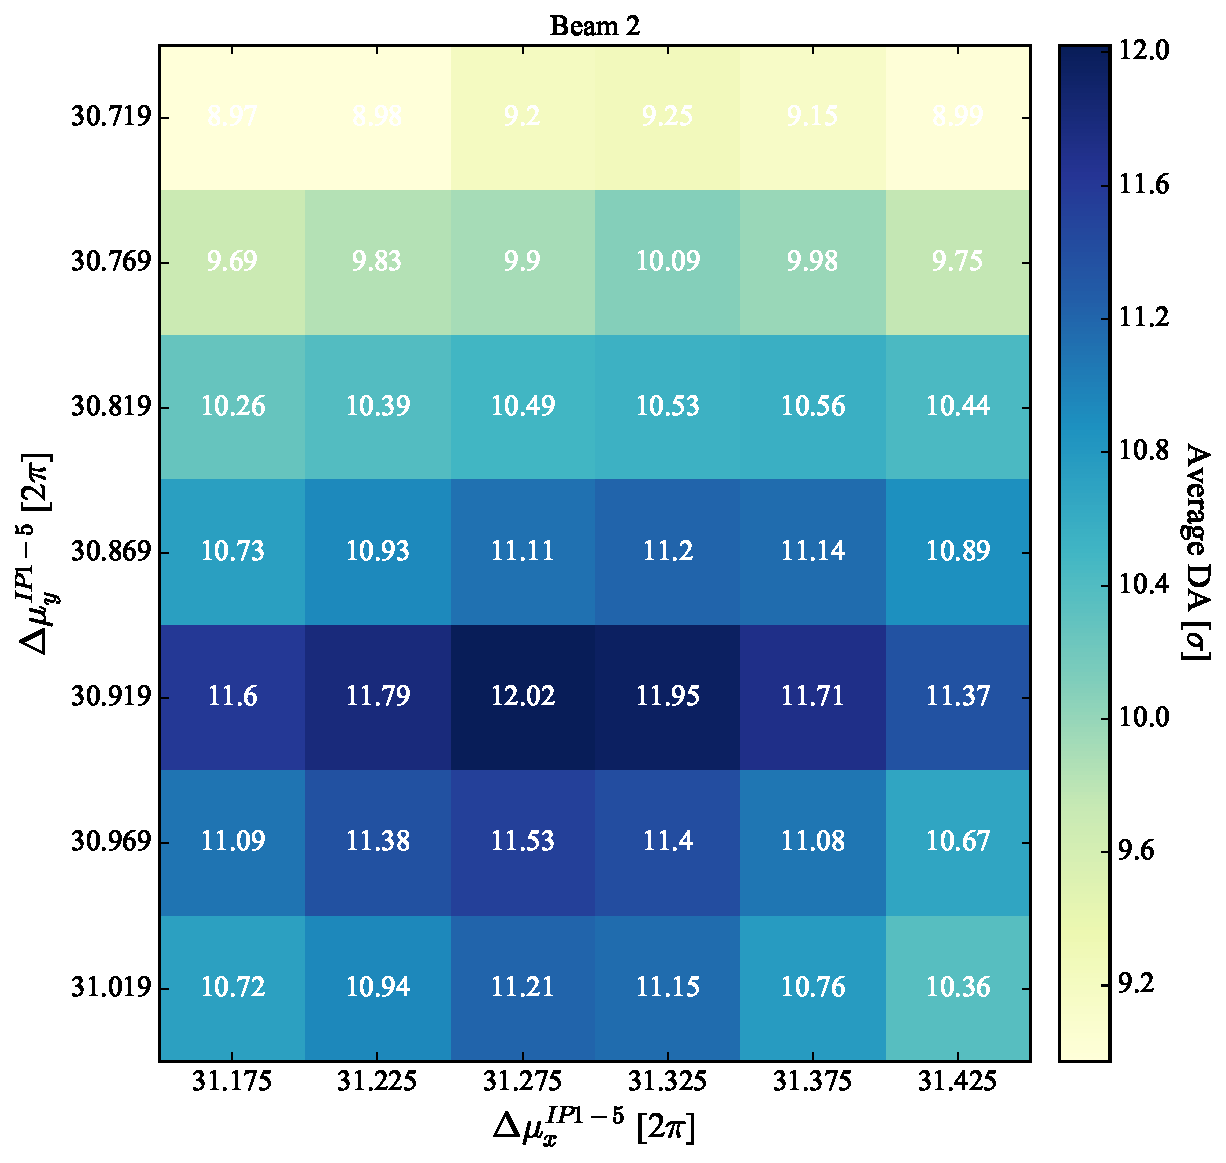
\includegraphics[width=0.49\textwidth]{images/scan_baseline_avg_b2.pdf} \\
\caption{\label{scan_da_base} Scan of the horizontal and vertical phase advance between IP1 and IP5 $\Delta\mu_{xy}^{IP1-5}$ as function of the average DA for Beam 1 (left plot) and Beam 2 (right plot). The DA is simulated without multipolar imperfections, with crossing angle, dispersion correction and Landau octupoles set to their maximum strength of -570 A, after 10$^{6}$ turns and calculated over 60 angles.}
\end{figure}


\begin{figure}[h!]
\centering
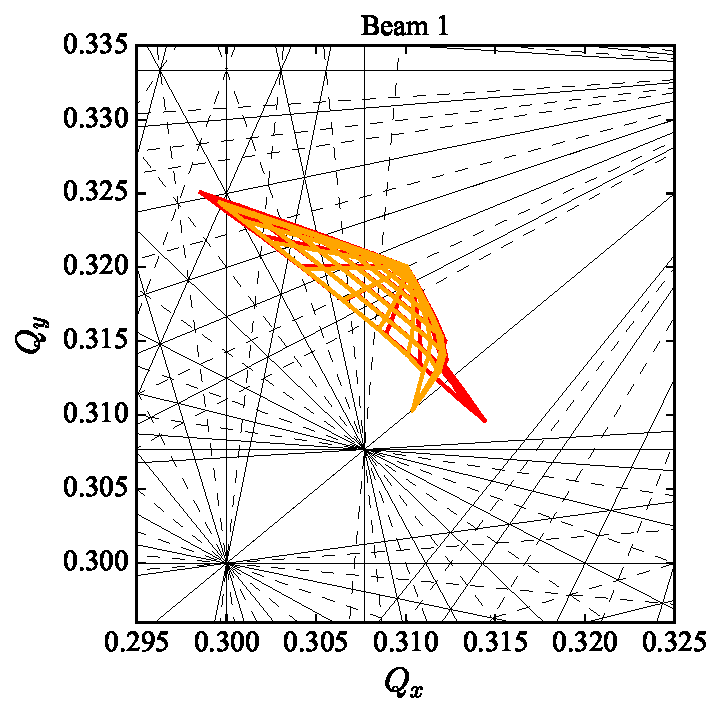
\includegraphics[width=0.49\textwidth]{images/footprint_b1_base_optim.pdf} \hfill 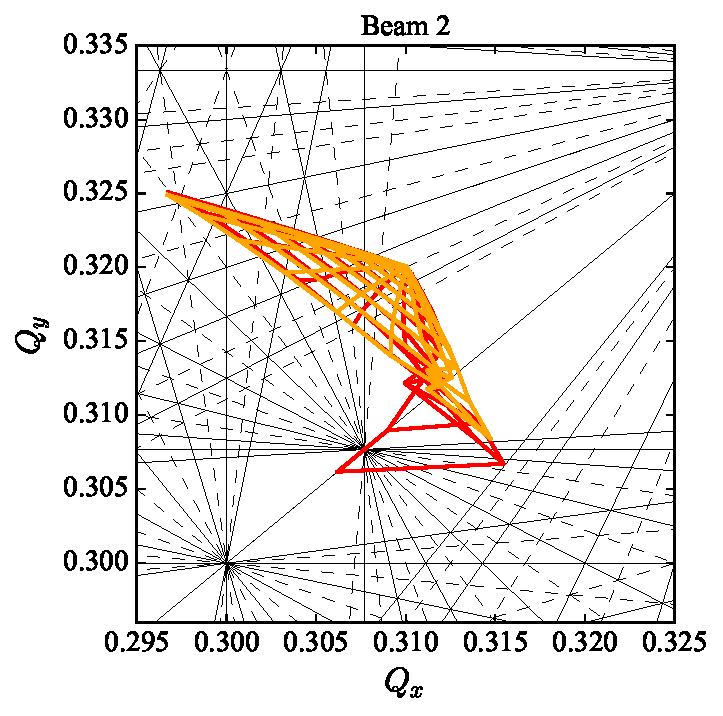
\includegraphics[width=0.49\textwidth]{images/footprint_b2_base_optim.pdf} \\
\caption{\label{footprint_optim} }
\end{figure}

\begin{figure}[h!]
\centering
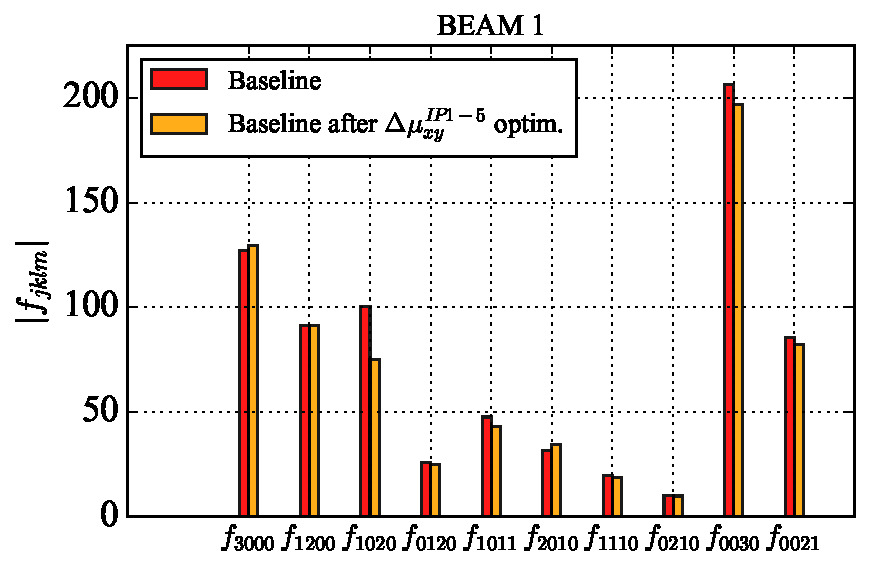
\includegraphics[width=0.49\textwidth]{images/rdt_sext_base_b1_570_ca.pdf} \hfill 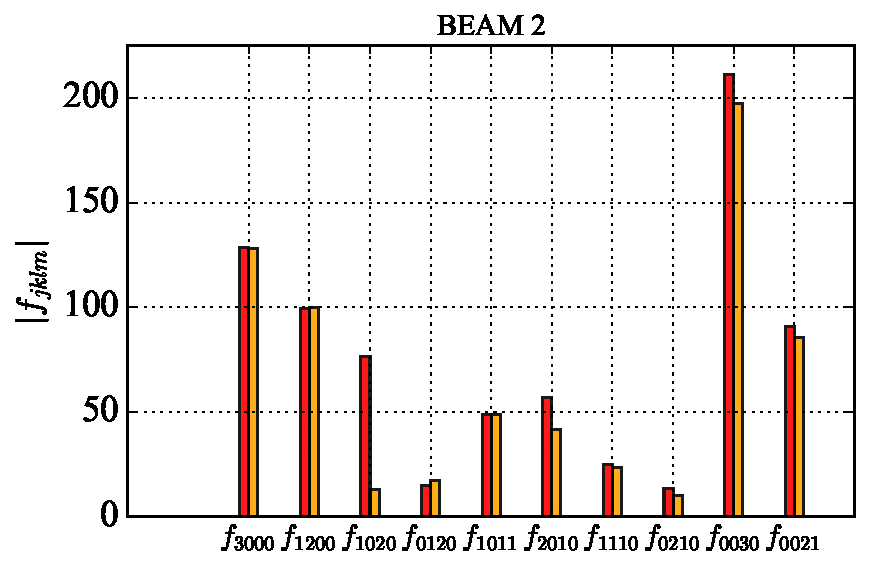
\includegraphics[width=0.49\textwidth]{images/rdt_sext_base_b2_570_ca.pdf} \\
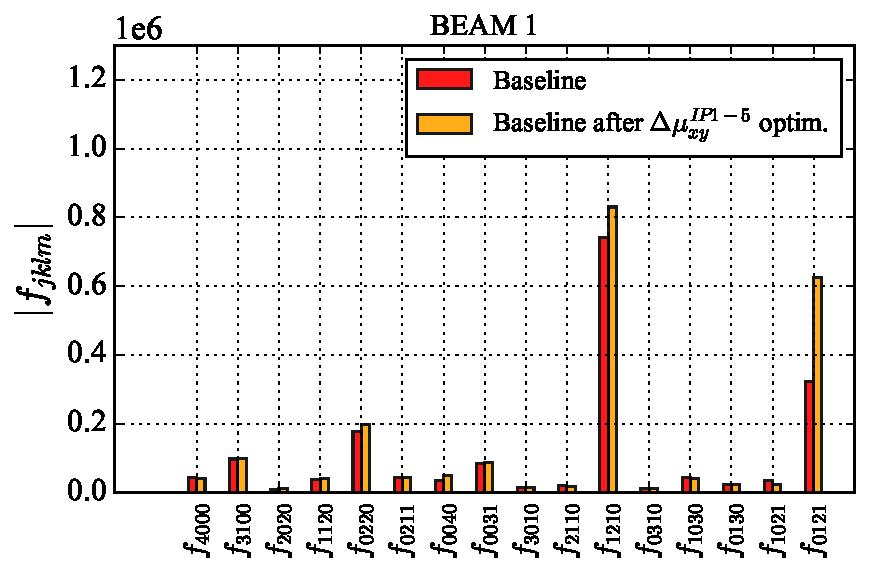
\includegraphics[width=0.49\textwidth]{images/rdt_oct_base_b1_570_ca.pdf} \hfill 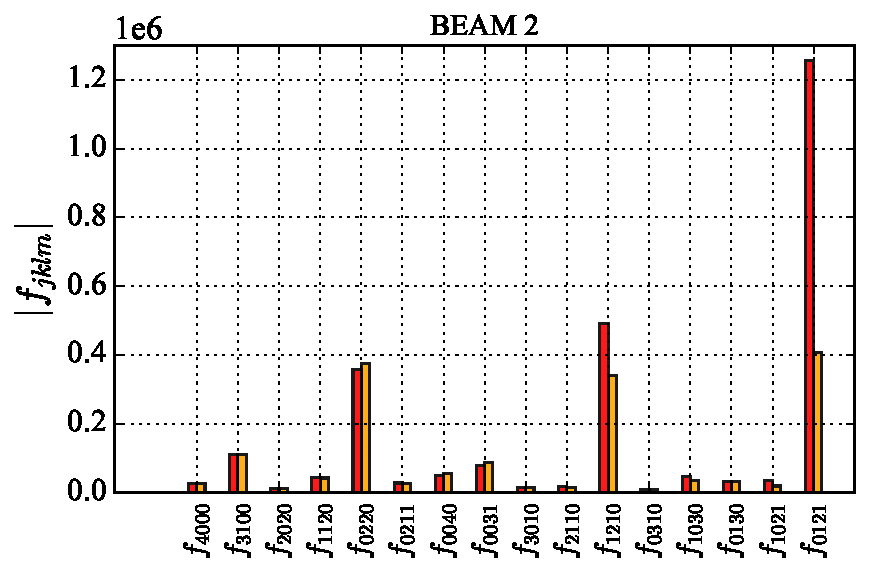
\includegraphics[width=0.49\textwidth]{images/rdt_oct_base_b2_570_ca.pdf}
\caption{\label{rdt_base} Average amplitude of the sextupole (top plots) and octupole (bottom plots) RDTs along the ring computed with PTC for Beam 1 (left plots) and Beam 2 (right plots) and with Landau octupoles set to -570 A.}
\end{figure}

\begin{figure}[h!]
\centering
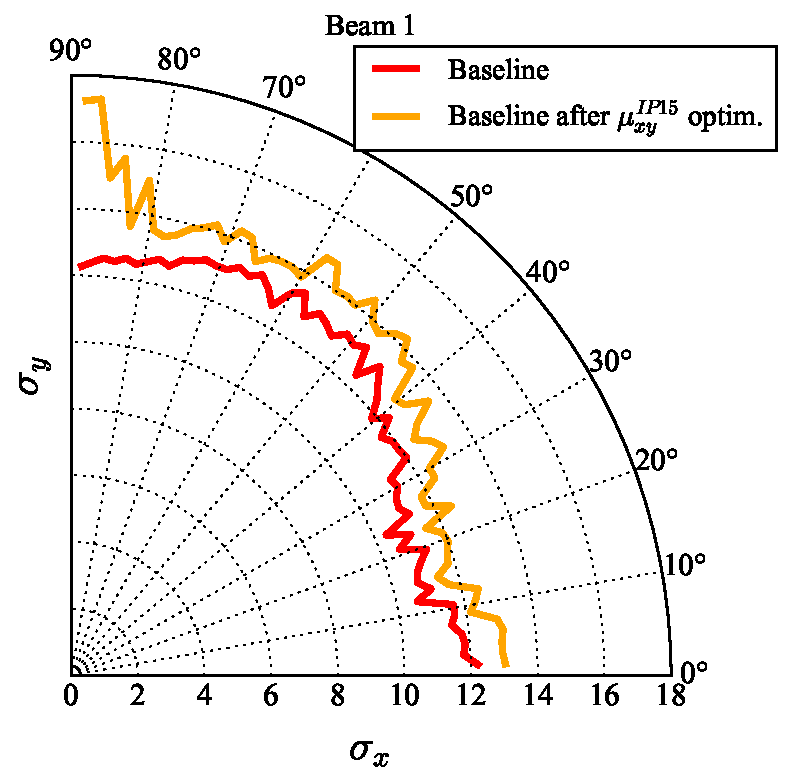
\includegraphics[width=0.47\textwidth]{images/da_polar_base_optim_b1.pdf} \hfill 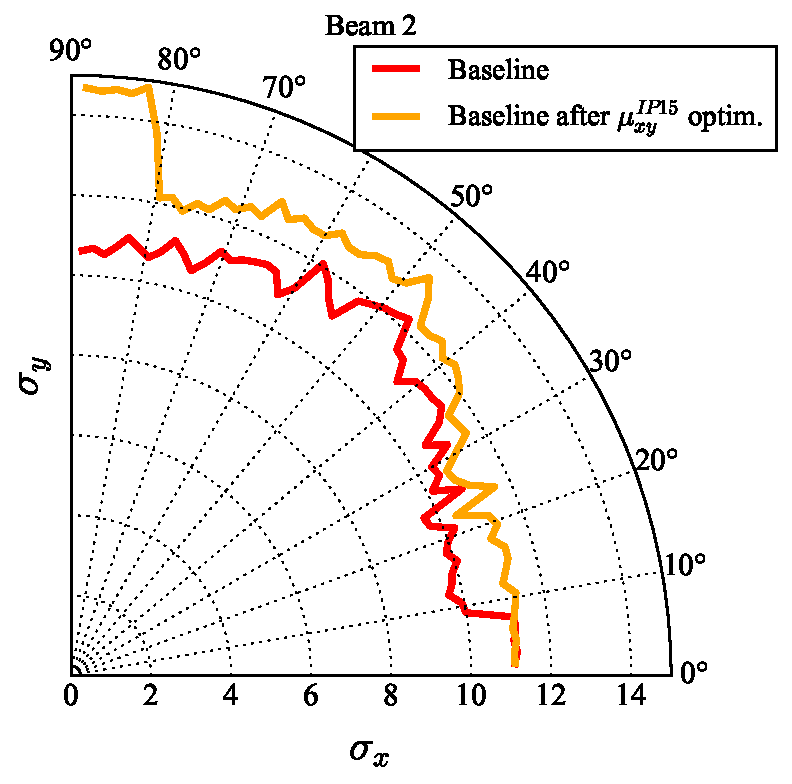
\includegraphics[width=0.47\textwidth]{images/da_polar_base_optim_b2.pdf}
\hbox{\hspace{1.0cm}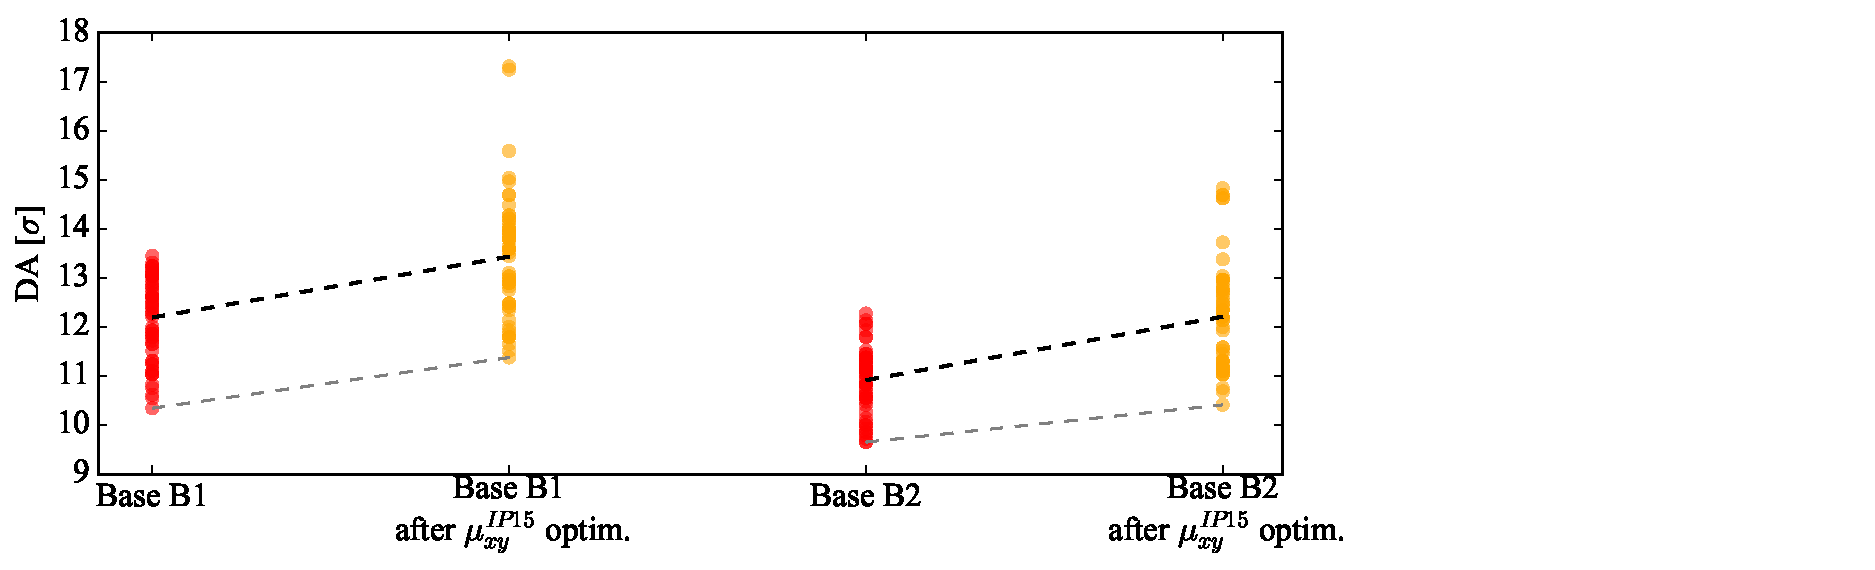
\includegraphics[width=1.2\textwidth]{images/da_noimp_base_b12.pdf}} 
\caption{\label{da_base} Dynamic aperture comparison before and after optimization of the horizontal and vertical phase advance between IP1 and IP5 $\Delta\mu_{xy}^{IP1-5}$ for Beam 1 and 2. The DA is simulated without multipolar imperfections, with crossing angle, dispersion correction and Landau octupoles set to their maximum strength of -570 A, after 10$^{6}$ turns and calculated over 60 angles. }
\end{figure}

\clearpage

\section{Alternative lattice sextupole optimization without MS10} \label{alternative}

No MS14F and No MS14F\&MS14D

\subsection{Sextupole layout and optics changes }

Phase change for No MS14F

\begin{figure}[h!]
\centering
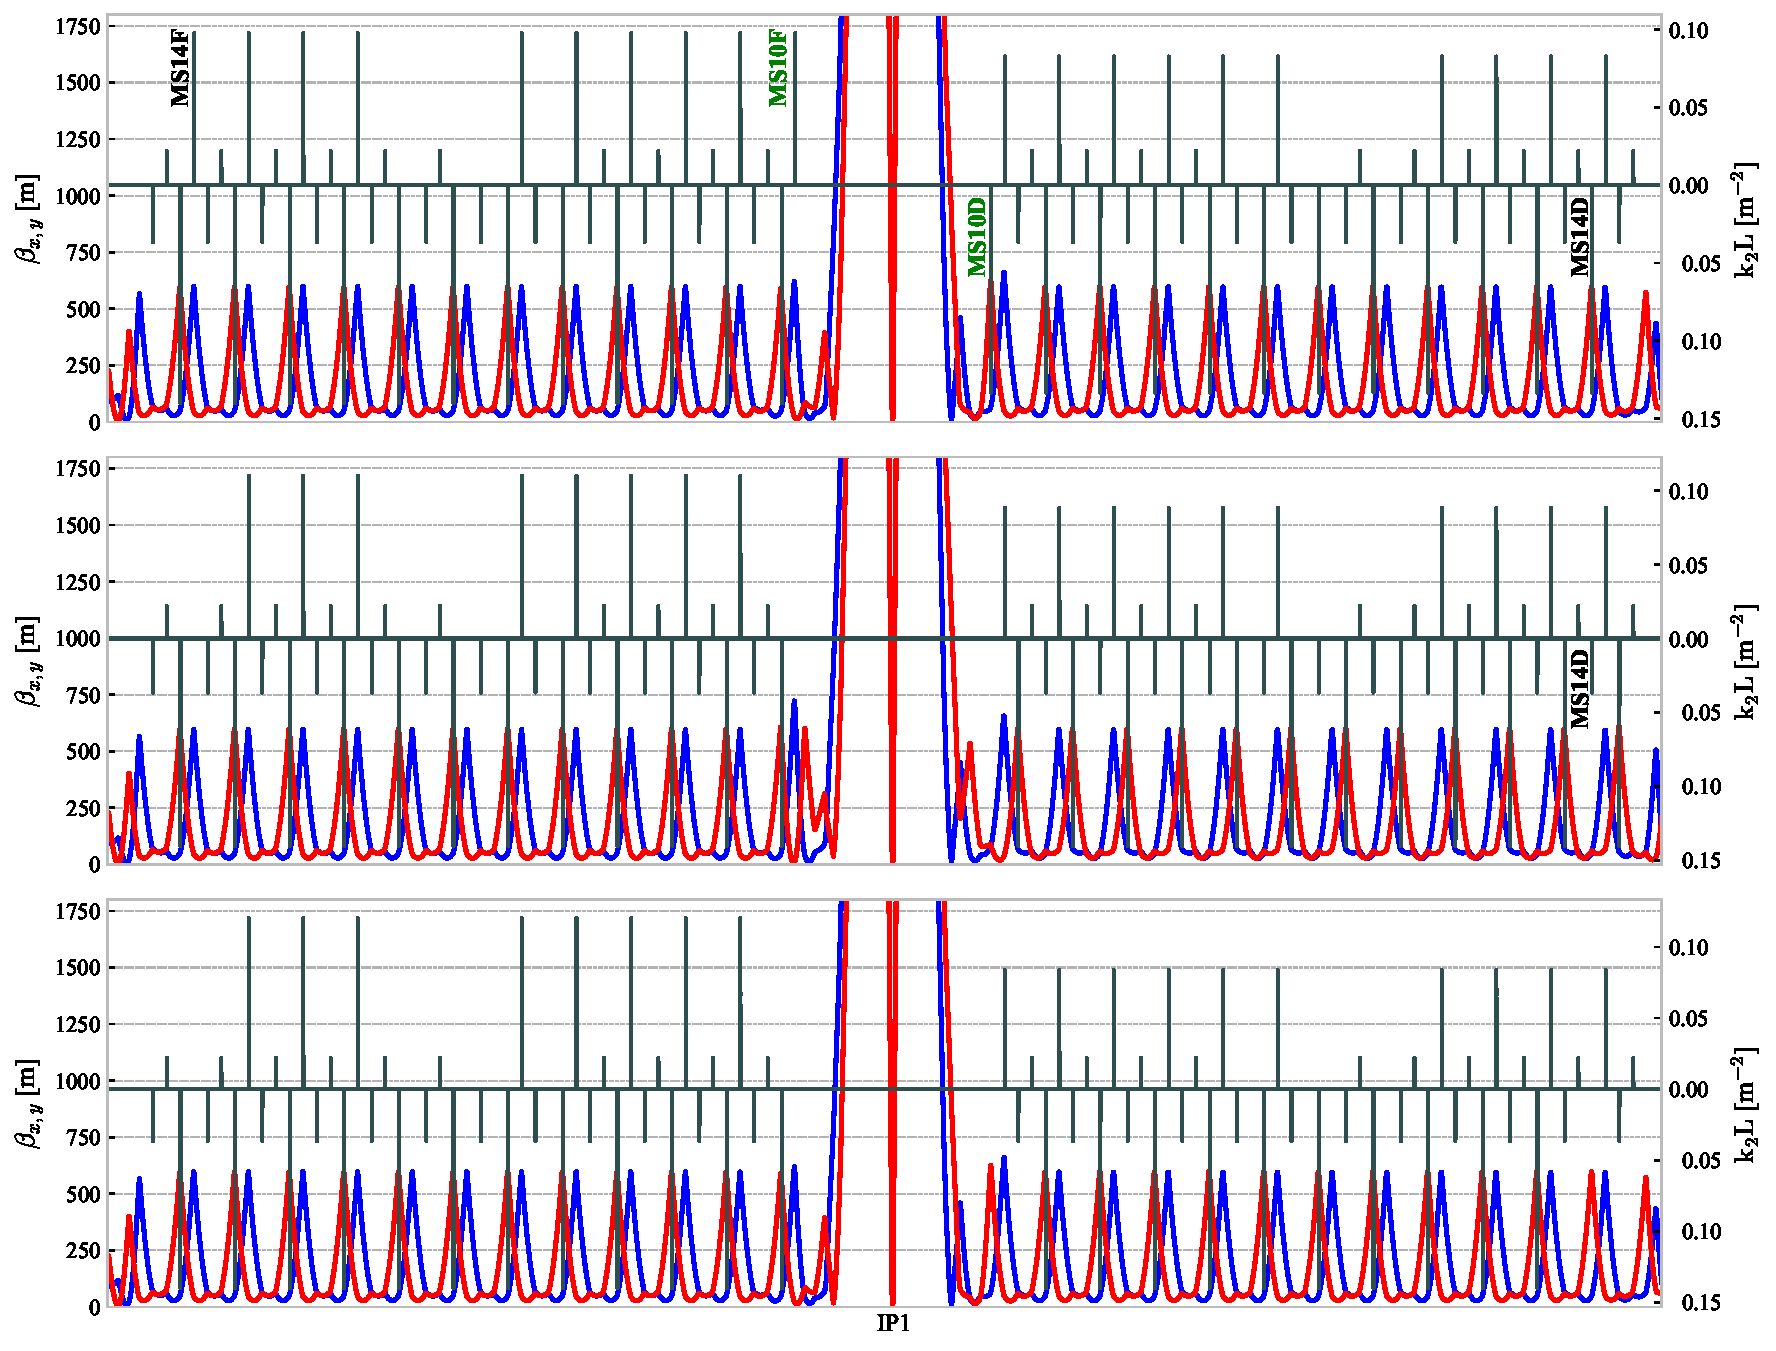
\includegraphics[width=1\textwidth]{images/twiss_k2l_allnoms10_b1.pdf}
\caption{\label{fig_twiss_all} Lattice sextupole configuration around IR1 of the Baseline, the No MS14F and the No MS14F \& MS14D optics.}
\end{figure}

\begin{figure}[h!]
\centering
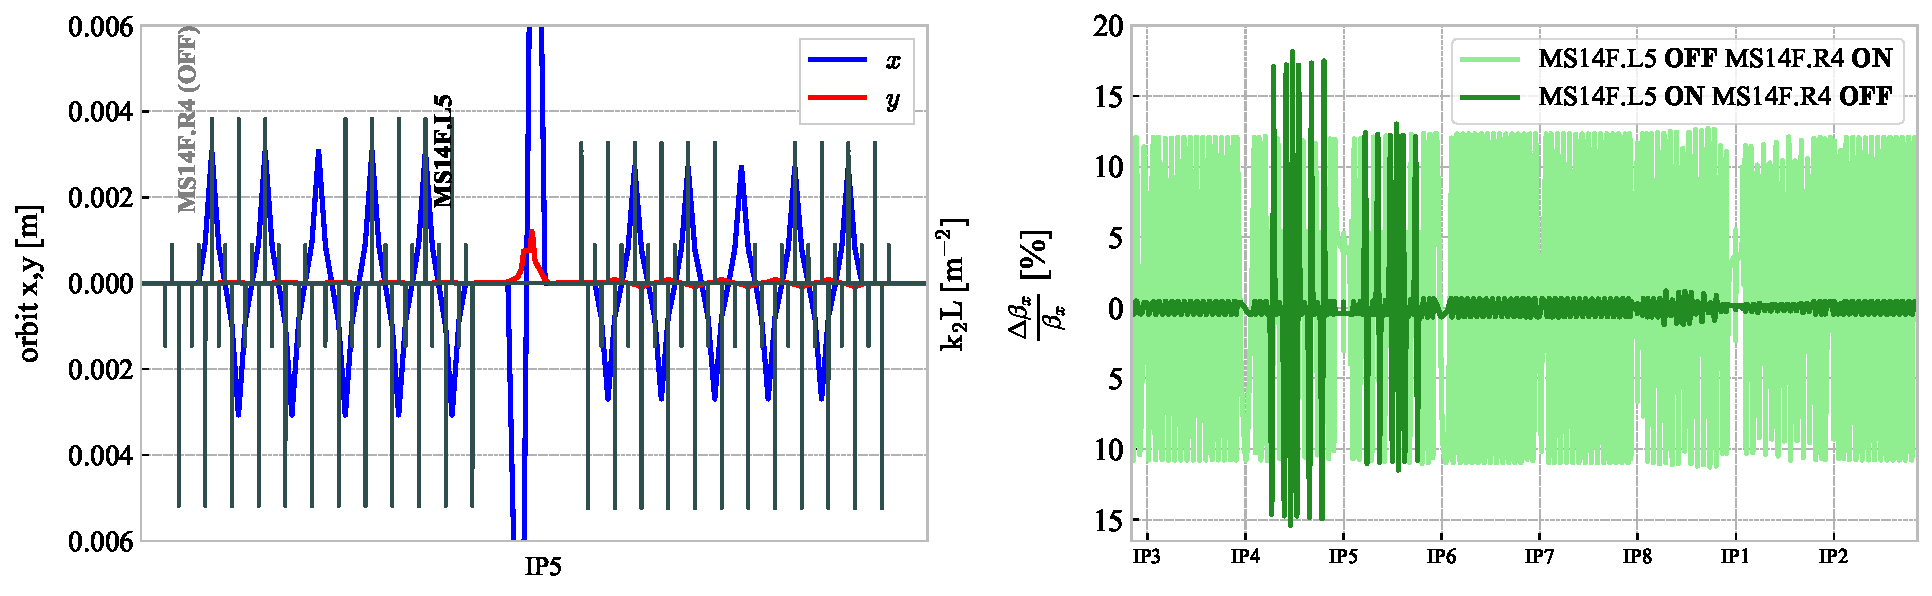
\includegraphics[width=1\textwidth]{images/ca_k2l_noms14falt_b1_ip5.pdf}\\
\caption{\label{noms14falt_optics} }
\end{figure}
%\begin{figure}[h!]
%\centering
%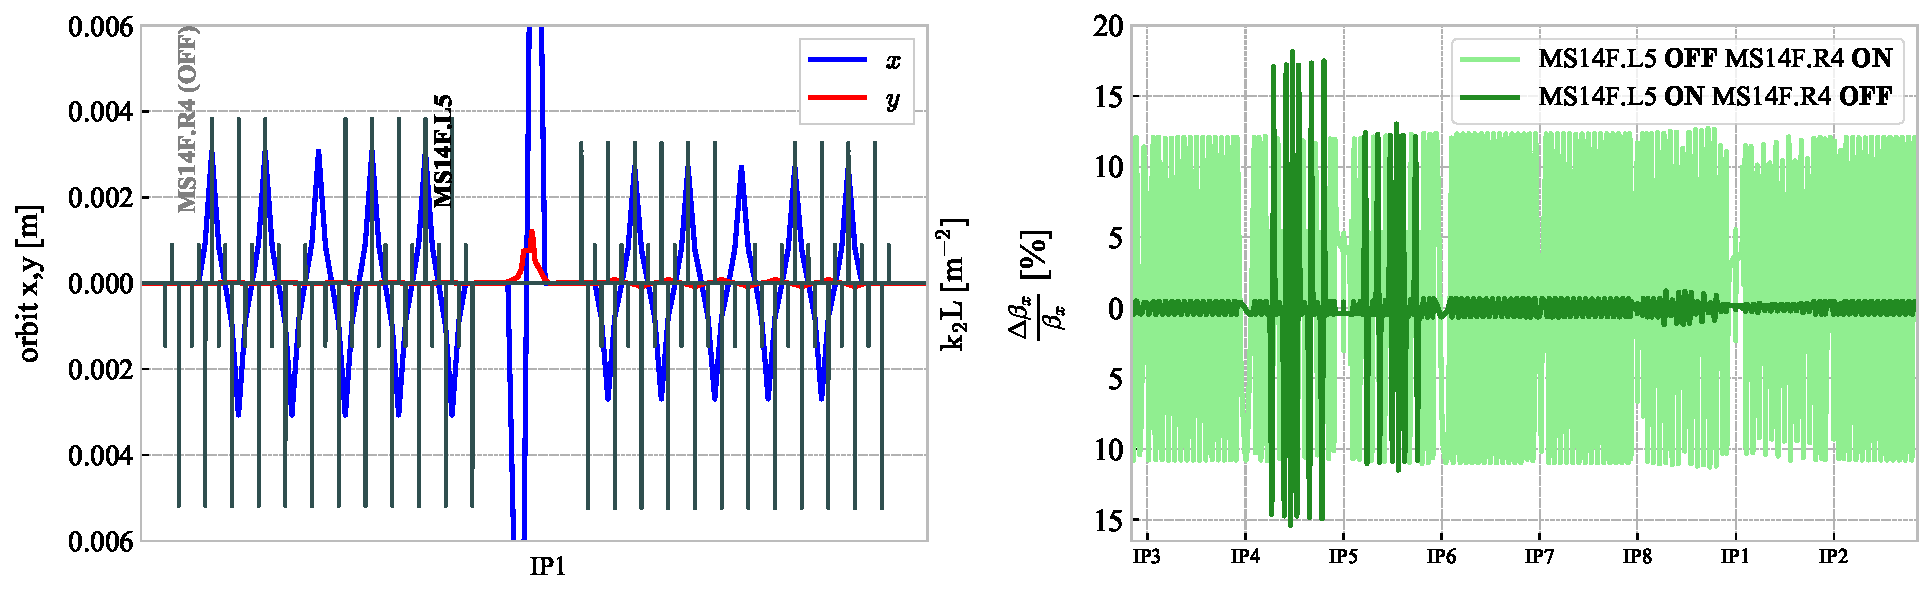
\includegraphics[width=0.49\textwidth]{images/ca_k2l_noms14falt_b1_ip1.pdf} \hfill 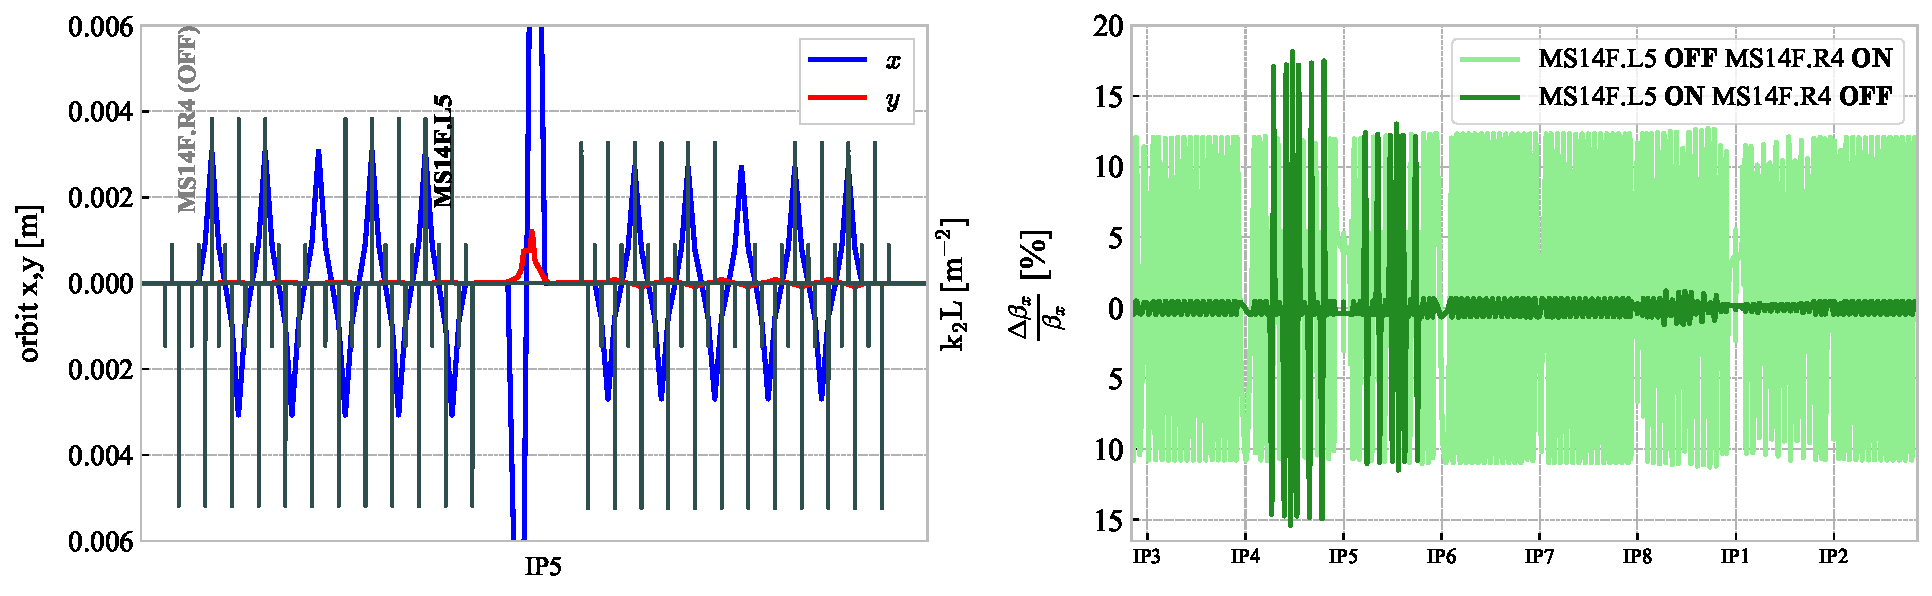
\includegraphics[width=0.49\textwidth]{images/ca_k2l_noms14falt_b1_ip5.pdf} \\
%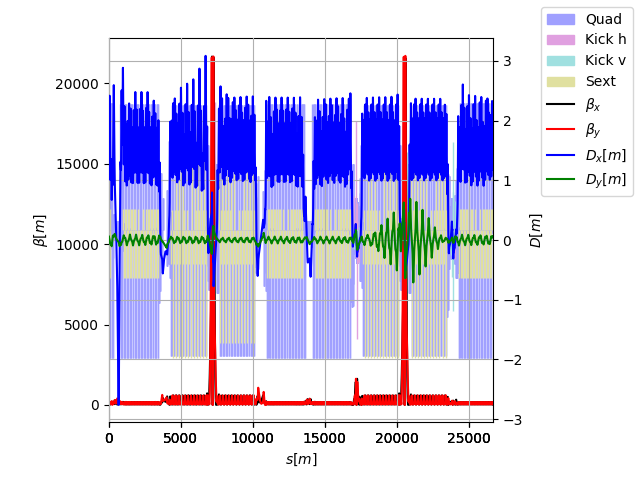
\includegraphics[width=0.55\textwidth]{images/dx_dy_noms14falt_b1.png} \hfill 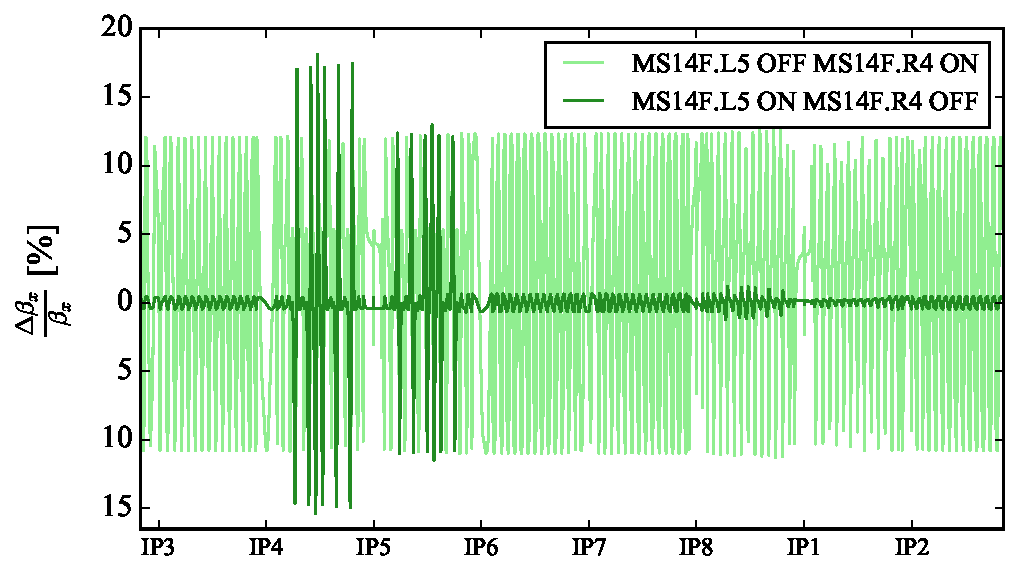
\includegraphics[width=0.42\textwidth]{images/bbeat_noms14falt_b1.pdf} \\
%\caption{\label{noms14falt_optics} }
%\end{figure}

\subsubsection{Geometrical aberrations}

Good correction of sextupolar rdts.

\begin{figure}[h!]
\centering
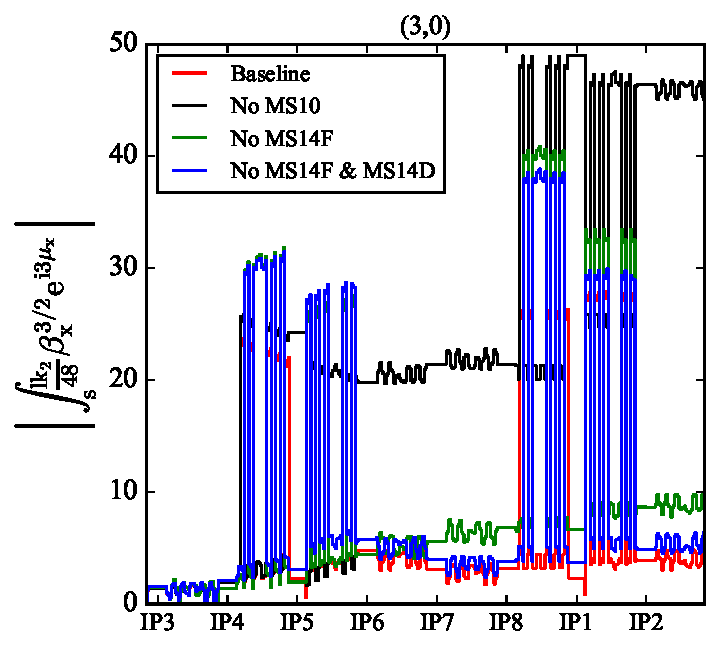
\includegraphics[width=0.49\textwidth]{images/3000_rdt_all_b1.pdf} \hfill 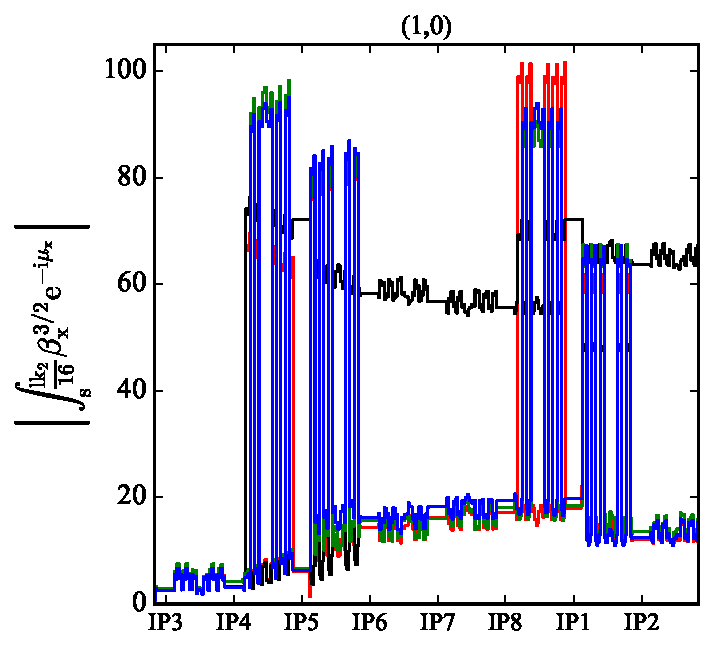
\includegraphics[width=0.49\textwidth]{images/1200_rdt_all_b1.pdf} \\
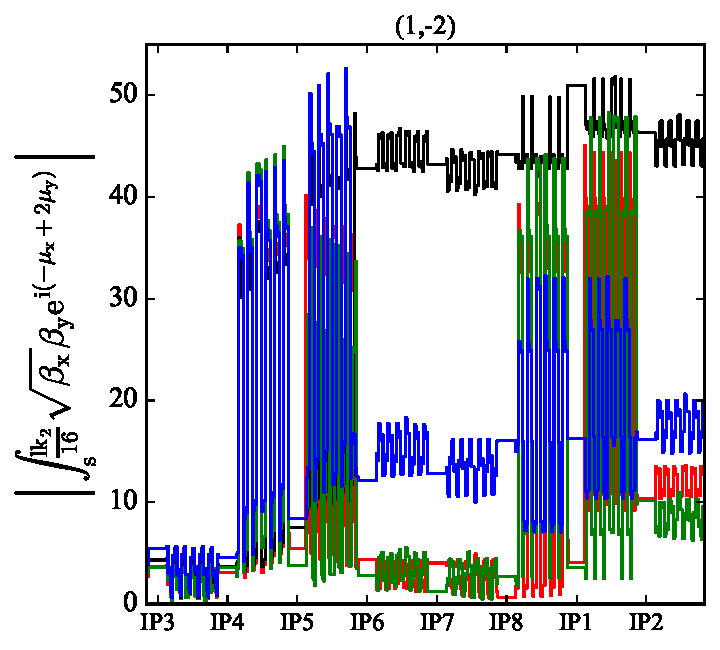
\includegraphics[width=0.49\textwidth]{images/0120_rdt_all_b1.pdf} \hfill 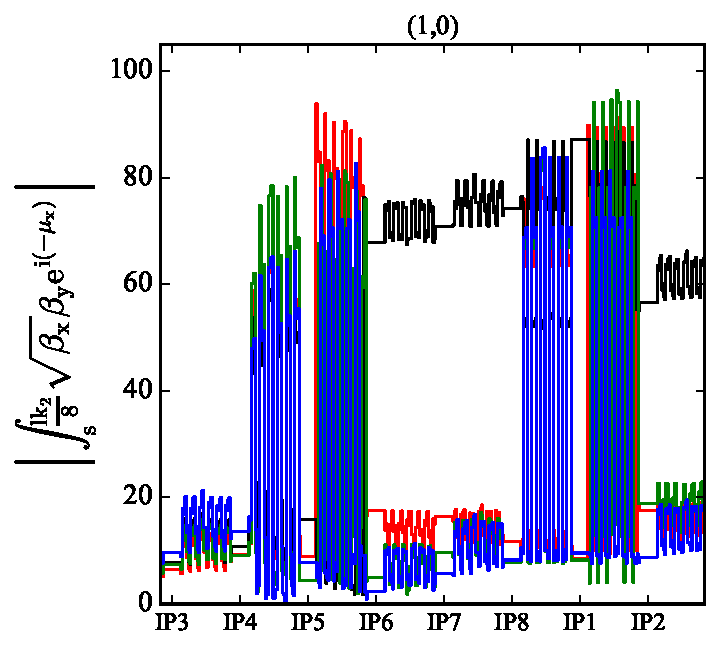
\includegraphics[width=0.49\textwidth]{images/0111_rdt_all_b1.pdf}
\caption{\label{rdt_twiss_all} Comparison of the sextupole geometrical RDTs along the ring for the different lattice sextupole options.}
\end{figure}


\subsection{DA improvement with $\Delta\mu_{xy}^{IP1-5}$}

DA comparison

\begin{figure}[h!]
\centering
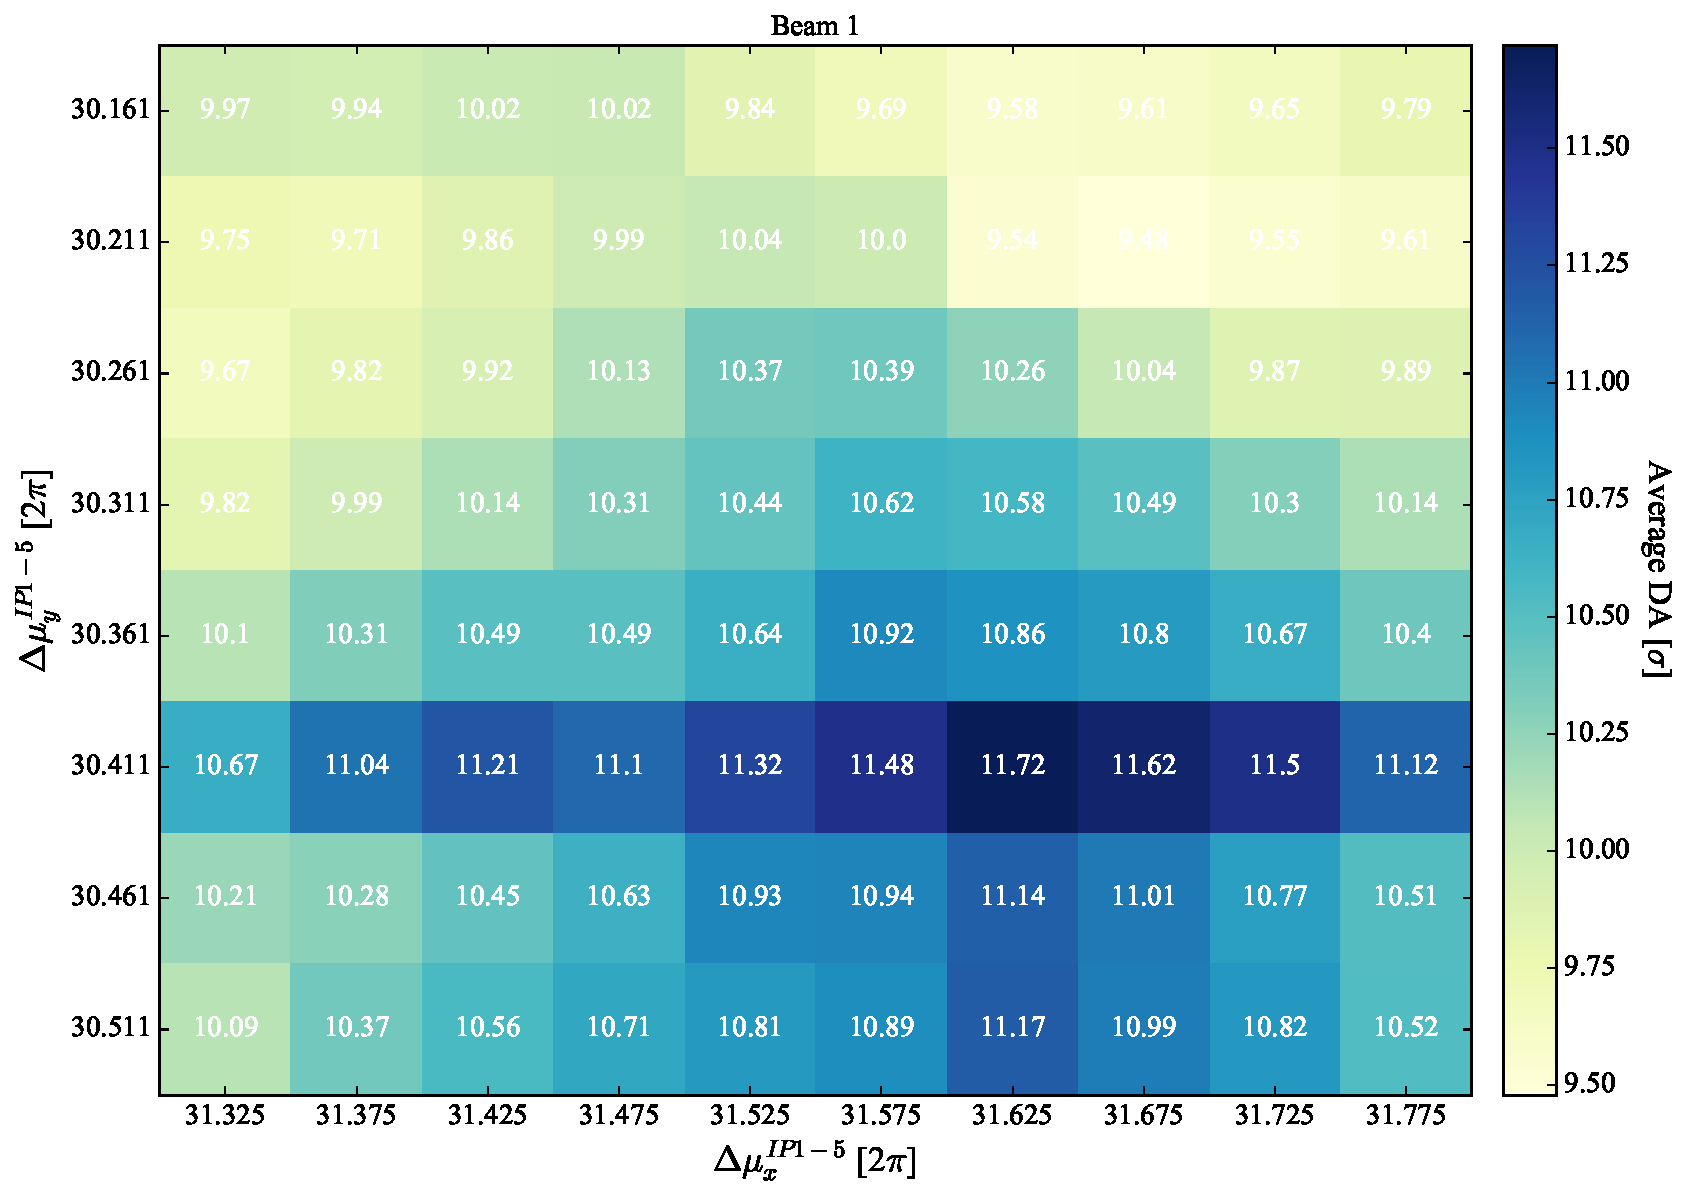
\includegraphics[width=0.8\textwidth]{images/scan_noms14falt_avg_b1.pdf} \\
\caption{\label{da_scan_ms14f} No MS14F optics: scan of the horizontal and vertical phase advance between IP1 and IP5 $\Delta\mu_{xy}^{IP1-5}$ as function of the average DA for Beam 1. }
\end{figure}

\begin{figure}[h!]
\centering
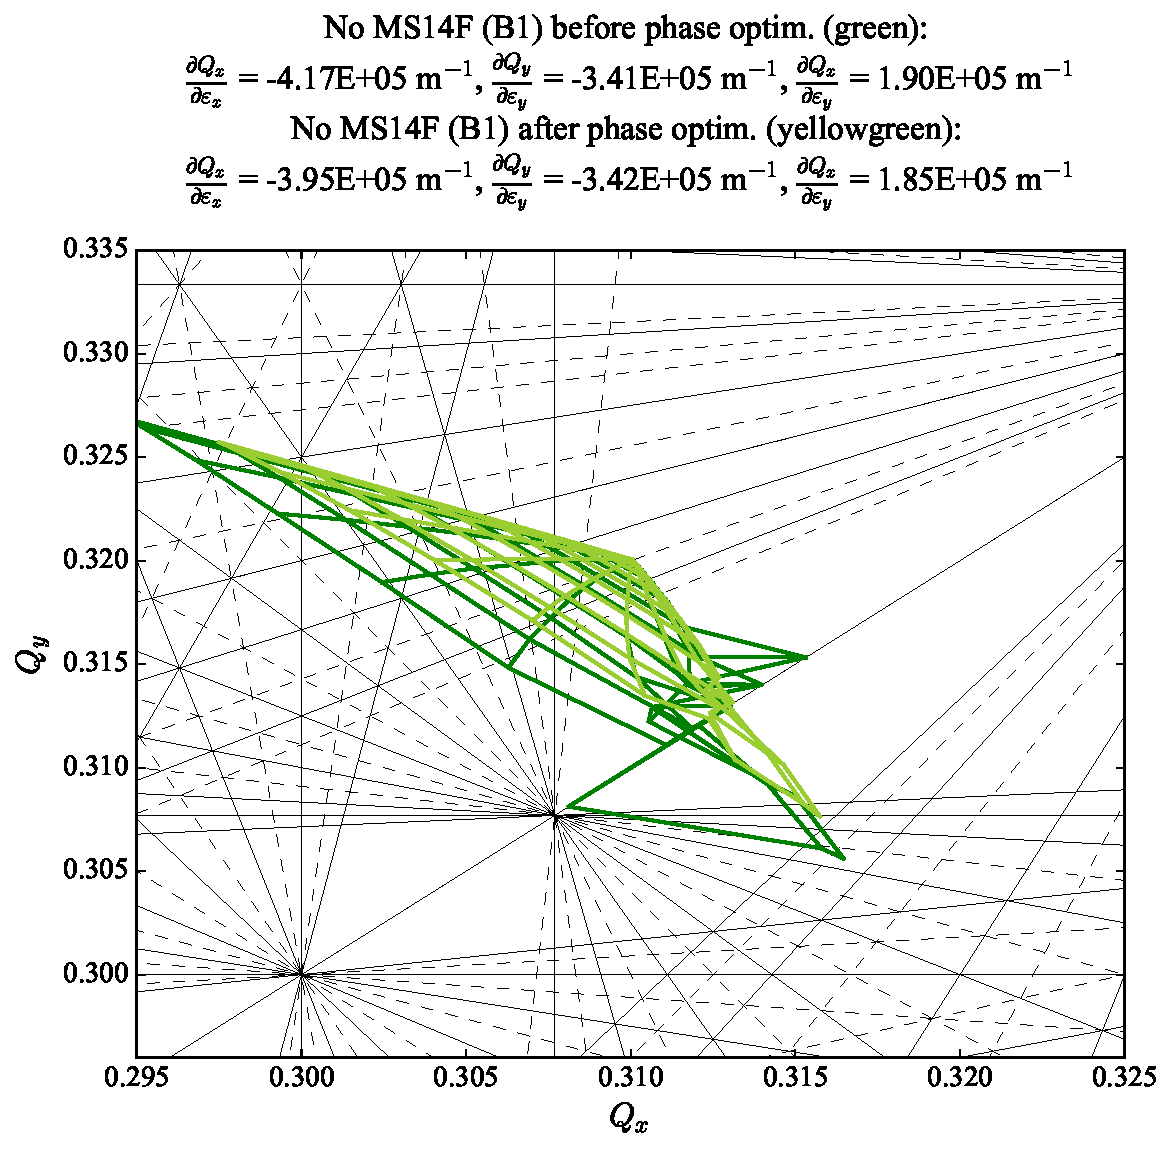
\includegraphics[width=0.6\textwidth]{images/footprint_b1_noms14falt_optim.pdf} \\
\caption{\label{da_scan_ms14f} No MS14F optics: Footprint (Beam 1) on the tune diagram with full crossing scheme, dispersion correction and $k_{\mathrm{MO}}$~=~-570~A. Comparison between the optics before $\Delta\mu_{xy}^{IP1-5}$ optimization (as studied in~\cite{ms10_ppt1}) and after optimization. }
\end{figure}


\begin{figure}[h!]
\centering
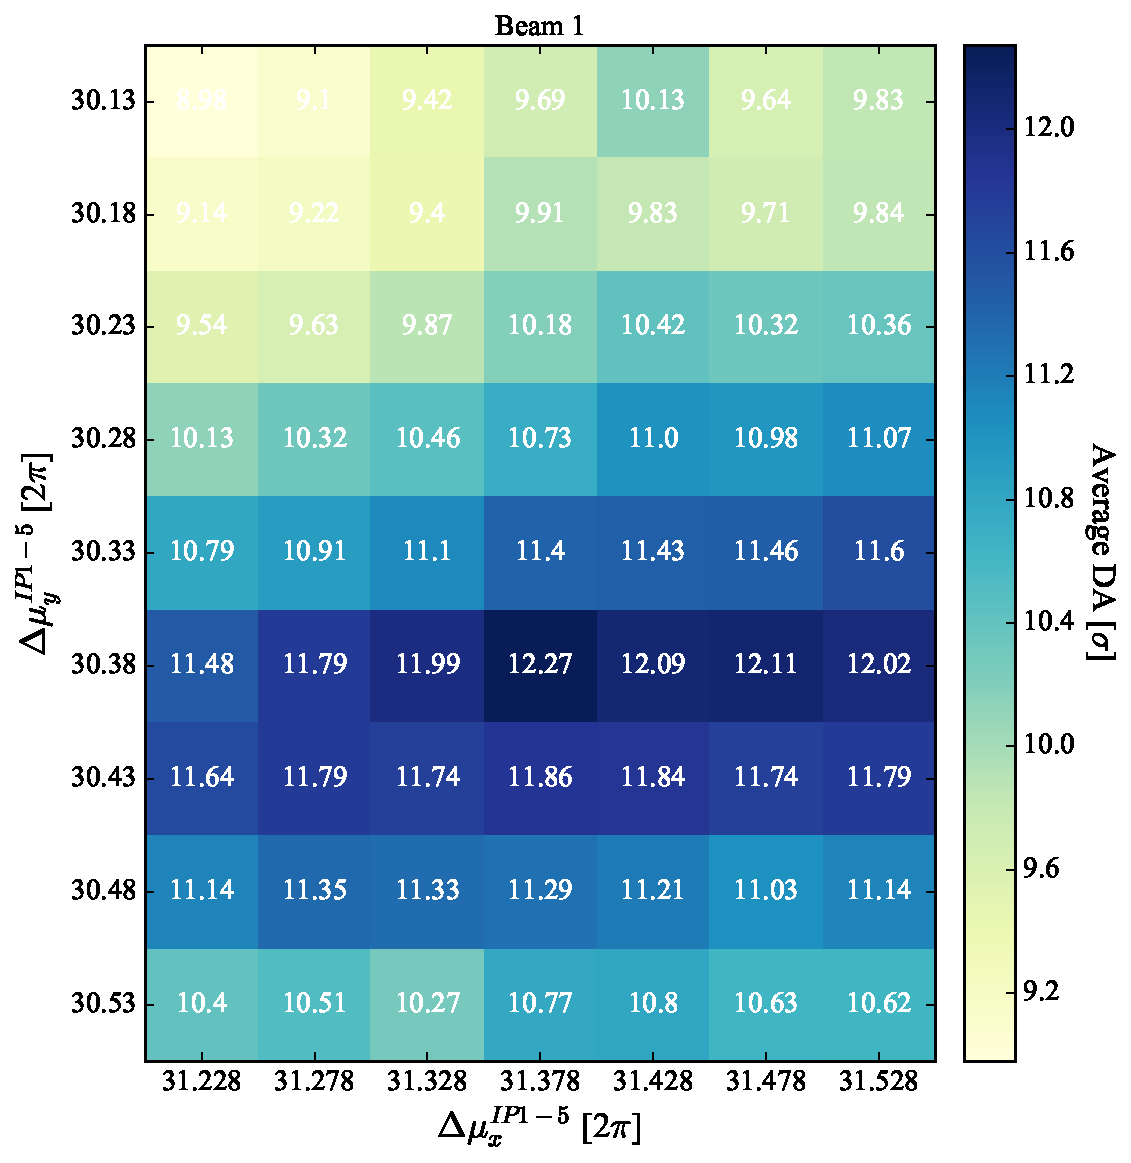
\includegraphics[width=0.49\textwidth]{images/scan_noms14fms14dalt_avg_b1.pdf} \hfill 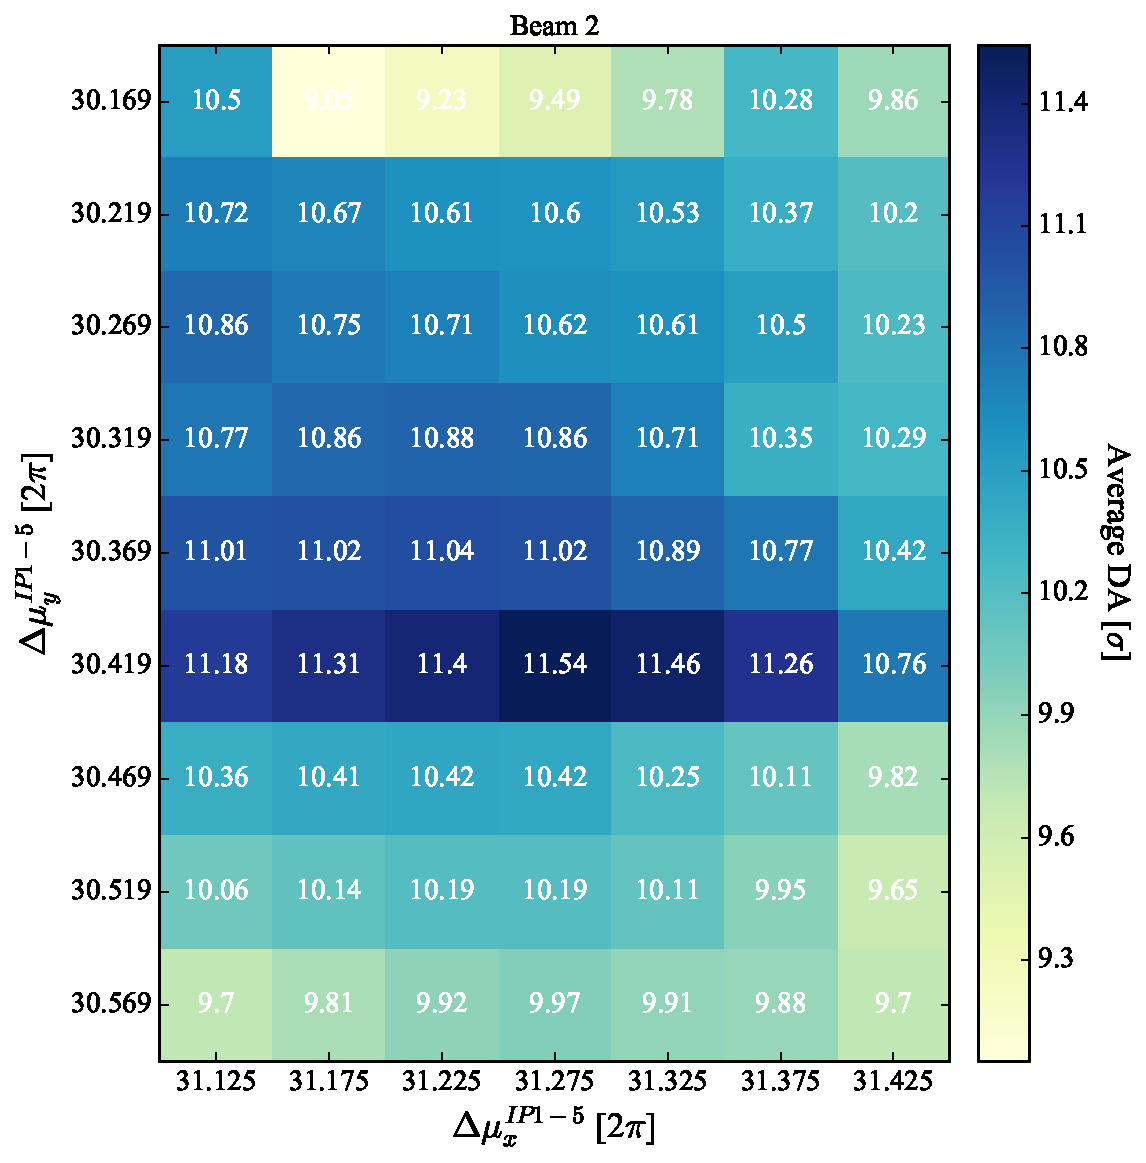
\includegraphics[width=0.49\textwidth]{images/scan_noms14fms14dalt_avg_b2.pdf} \\
\caption{\label{da_scan_ms14fms14d} No MS14F \& MS14D optics: scan of the horizontal and vertical phase advance between IP1 and IP5 $\Delta\mu_{xy}^{IP1-5}$ as function of the average DA for Beam 1 (left plot) and Beam 2 (right plots).}
\end{figure}


\begin{figure}[h!]
\centering
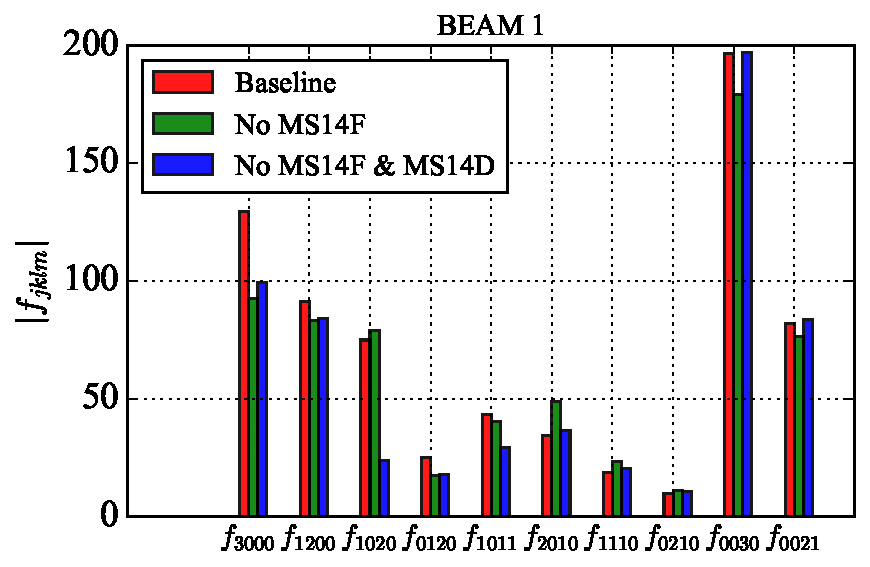
\includegraphics[width=0.49\textwidth]{images/rdt_sext_optics_compare_b1_570_noca.pdf} \hfill 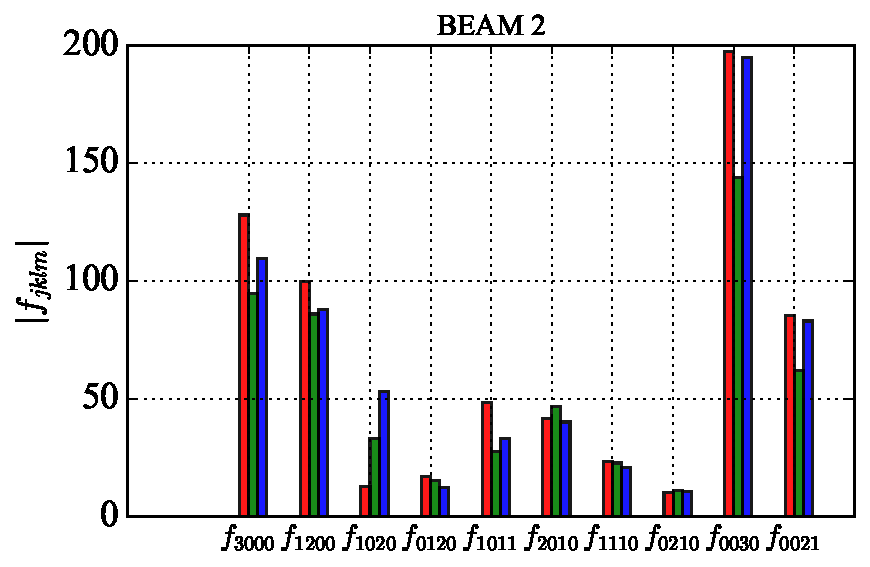
\includegraphics[width=0.49\textwidth]{images/rdt_sext_optics_compare_b2_570_noca.pdf} \\
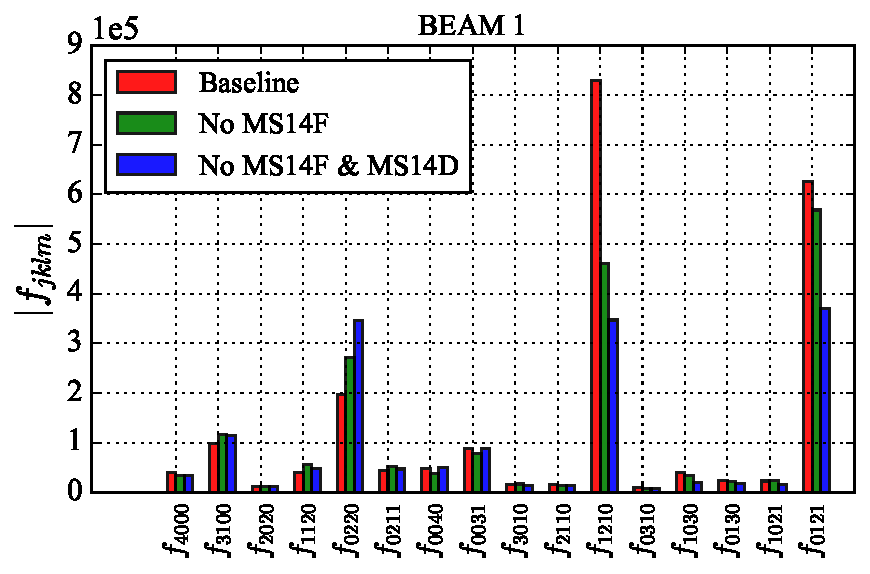
\includegraphics[width=0.49\textwidth]{images/rdt_oct_optics_compare_b1_570_noca.pdf} \hfill 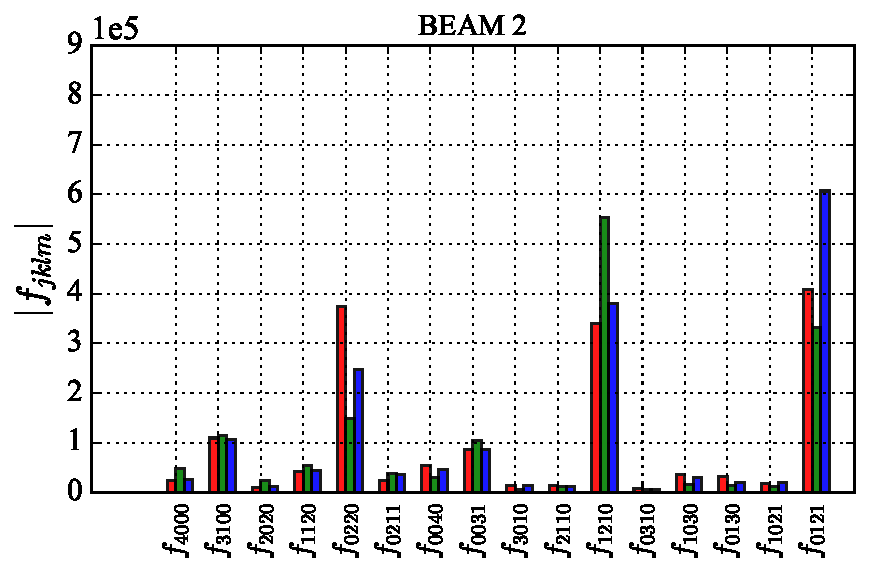
\includegraphics[width=0.49\textwidth]{images/rdt_oct_optics_compare_b2_570_noca.pdf}
\caption{\label{rdt_ptc_all} Average amplitude, after $\Delta\mu_{xy}^{IP1-5}$ optimization, of the sextupole (top plots) and octupole (bottom plots) RDTs along the ring computed with PTC for Beam 1 (left plots) and Beam 2 (right plots) and with Landau octupoles set to -570 A.}
\end{figure}


\subsubsection{Footprint}

FMA for B1 and B2 on all optics.

\begin{figure}[h!]
\centering
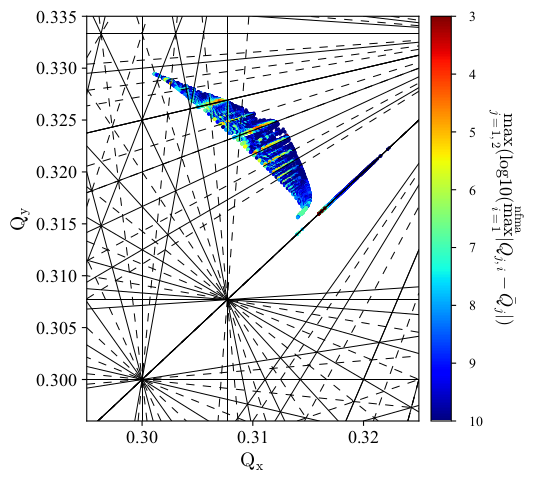
\includegraphics[width=0.49\textwidth]{images/fma_baseb1.png} \hfill 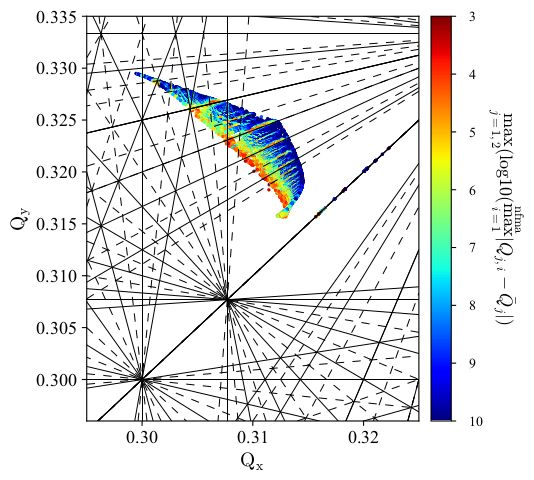
\includegraphics[width=0.49\textwidth]{images/fma_baseb2.png} \\
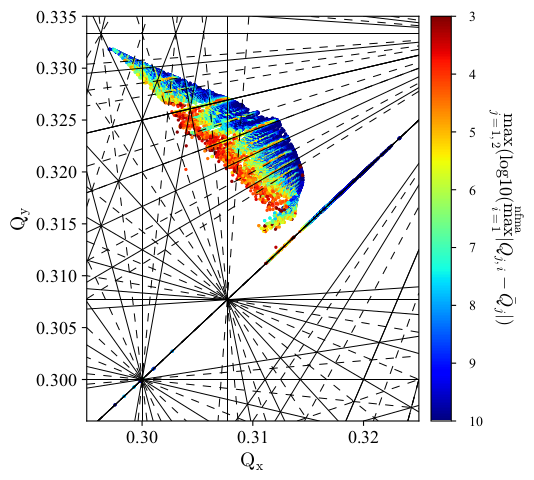
\includegraphics[width=0.49\textwidth]{images/fma_noms14faltb1.png} \hfill \includegraphics[width=0.49\textwidth]{images/fma_noms14faltb2.png} \\
\includegraphics[width=0.49\textwidth]{images/fma_noms14fms14daltb1.png} \hfill \includegraphics[width=0.49\textwidth]{images/fma_noms14fms14daltb2.png} \\
\caption{\label{fma_all} Frequency Map Analysis on Beam 1 (left plots) and Beam 2 (right plots) for the Baseline, No MS14F and No MS14F \& MS14D optics.}
\end{figure}

\subsubsection{Linear amplitude detuning}

Detuning with amplitude as function of octupole strength.

\begin{figure}[h!]
\centering
\includegraphics[width=0.31\textwidth]{images/qxjx_all_b1_ca.pdf}\hfill \includegraphics[width=0.31\textwidth]{images/qyjy_all_b1_ca.pdf}\hfill \includegraphics[width=0.31\textwidth]{images/qxjy_all_b1_ca.pdf} \\
\includegraphics[width=0.31\textwidth]{images/qxjx_all_b2_ca.pdf}\hfill \includegraphics[width=0.31\textwidth]{images/qyjy_all_b2_ca.pdf}\hfill \includegraphics[width=0.31\textwidth]{images/qxjy_all_b2_ca.pdf} \\
\caption{\label{amp_det_all} }
\end{figure}


\subsubsection{Chromatic properties}

Impact on chromaticity and chromatic $\beta$-beating.

\begin{figure}[h!]
\centering
\includegraphics[width=0.49\textwidth]{images/qxy_vs_dp_all_b1.pdf} \hfill \includegraphics[width=0.49\textwidth]{images/qxy_vs_dp_all_b2.pdf}
\caption{\label{q_vs_dp_all} Tunes versus energy for Beam 1 (left plot) and Beam 2 (right plot). }
\end{figure}

\begin{figure}[h!]
\centering
\includegraphics[width=0.49\textwidth]{images/twiss_wx_all_b1.pdf} \hfill \includegraphics[width=0.49\textwidth]{images/twiss_wy_all_b1.pdf}
\caption{\label{w_all} Amplitude of the chromatic $\beta$-beating along the machine for the different sexupole lattice options. }
\end{figure}


\subsubsection{DA comparison}

DA

\begin{figure}[h!]
\centering
\includegraphics[width=1\textwidth]{images/da_polar_all_b12.pdf}\\
\hbox{\hspace{0.0cm}\includegraphics[width=1.0\textwidth]{images/da_all_b12.pdf}}
\caption{\label{da_final_all} Dynamic aperture after $\Delta\mu_{xy}^{IP1-5}$ optimization for Beam 1 and 2. The DA is simulated without multipolar imperfections, with crossing angle, dispersion correction and Landau octupoles set to their maximum strength of -570 A, after 10$^{6}$ turns and calculated over 60 angles. }
\end{figure}


\subsection{IR6 constraints}

Constraints imposed by the machine protection.

\begin{table}[h!]
\begin{center}
\caption{\label{tab_circuit_ms10} IR6 main parameters comparison for the different proposed optics (after $\Delta\mu_{xy}^{IP1-5}$ optimization).}
\begin{tabular}{lcccc} \hline
Param. B1 / B2 &  Target values  &   Baseline    &    No MS14F     &   No MS14F\&MS14D  \\ \hline
$\Delta\mu_{x,\mathrm{MKD-TCDQ}}$ [$^{\circ}$]  &  90$^{\circ} \pm$ 4$^{\circ}$  &    86.3 / 93.6   &     91.5 / 93.6    &    86.3 / 93.6  \\ 
$\beta_{y}^{\mathrm{TCDS}}$       [m]       &  $\geq$ 200            &    238.3 / 260.6   &  283.2 / 200.0   &    238.3 / 271.0   \\
$\beta_{x}^{\mathrm{TCDQ}}$       [m]       &   -             &    736.4 / 473.3   &  513.9 / 460.0   &    736.4 / 474.6   \\
$\beta_{y}^{\mathrm{TCDQ}}$       [m]       &  $\geq$145                   &    180.5 / 145.0  &  145.0 / 176.2   &    180.5 / 145.0   \\
$|\mathrm{D}_{x,\mathrm{TCDQ}}|$  [m]       &   -                 &    0.6 / 0.4       &     0.02 / 0.38  &    0.5 / 0.42       \\ 
Gap$_{\mathrm{TCQD,min}}$   [mm]       &    $\geq$3                 &    4.0 / 3.05      &    3.3  / 2.99  &    4.0 /3.05        \\ 
$\beta_{x}^{\mathrm{TDE}}$        [km]      &  $\geq$4                     &    6.37 / 4.92   &  5.06 / 4.83   &    6.37 / 4.93   \\
$\beta_{y}^{\mathrm{TDE}}$        [km]      &  $\geq$3.2                     &    3.36 / 7.23   &  8.2 / 6.33   &    3.36 / 7.72   \\
$(\beta_{x}\beta_{y})_{\mathrm{TDE}}^{\frac{1}{2}}$ [km] &       $\geq$4.5          &   4.62 / 5.98   &  6.44 / 5.53   &    4.62 / 6.17   \\
$|\Delta\mu_{x,\mathrm{MKD-TCT,\small{IP1}}}|$ [$^{\circ}$]  &    $\leq$20          &    19.8 / 18.8   &  9.8 / 18.6   &    5.0 / 19.6   \\        
$|\Delta\mu_{x,\mathrm{MKD-TCT,\small{IP5}}}|$ [$^{\circ}$]  &    $\leq$30          &    29.5 / 31.4   &  36 / 30.1   &    29.5 / 31.9   \\        
Q5.L6 [T/m]                                 &   160                        &            163 / -164             &           160 / -162                   &         163 / -165                     \\
Q5.R6 [T/m]                                 &   160                        &            -159 /  151      &               -161 / 151               &            -159 / 152                  \\ \hline

\end{tabular}
\end{center}
\end{table}

\clearpage

\subsection{Lattice optimization with only focusing or defocusing MS10}

Similar performance as for the Baseline optics was found with only one MS10 in each IR1 and IR5 instead of two. One can either move the MS14D to the MS10F location without using any additional sextupole or disconnect MS14D and install a new MS10F, depending on the technical complexity, time and cost. A second configuration would consist in disconnecting MS14F and add an MS10D. Both options restore an even number of sextupoles on each side of IP1 and IP5 while keeping the same total number of sextupole as the current LHC sextupole lattice. 

\begin{figure}[h!]
\centering
\includegraphics[width=1\textwidth]{images/twiss_k2l_noms10fdms14fd_b1.pdf}
\caption{\label{fig_twiss_all} Lattice sextupole configuration around IR1 of the No MS10D \& MS14D optics.}
\end{figure}

\begin{figure}[h!]
\centering
\includegraphics[width=1\textwidth]{images/da_polar_1addsext_b12.pdf} \\
\includegraphics[width=1\textwidth]{images/da_1addsext_b12.pdf}
\caption{\label{da_final_all} Dynamic aperture after $\Delta\mu_{xy}^{IP1-5}$ optimization for Beam 1 and 2. The DA is simulated without multipolar imperfections, with crossing angle, dispersion correction and Landau octupoles set to their maximum strength of -570 A, after 10$^{6}$ turns and calculated over 60 angles. }
\end{figure}

%\subsection{DA improvement}
%\subsection{Impact on optics and aberrations}


\section{DA with beam-beam}

\begin{figure}[h!]
\centering
\includegraphics[width=0.49\textwidth]{images/q_vs_da_Base_muxy_0.png} \hfill \includegraphics[width=0.49\textwidth]{images/q_vs_da_Base_muxy_optim.png} \\
\caption{\label{da_scan_ms14fms14d} Baseline optics: scan of the horizontal and vertical tunes before (left) and after (right) phase advance optimization between IP1 and IP5 $\Delta\mu_{xy}^{IP1-5}$ for Beam 1.}
\end{figure}
\begin{figure}[h!]
\centering
\includegraphics[width=0.49\textwidth]{images/q_vs_da_noms10_muxy_0.png} \hfill \includegraphics[width=0.49\textwidth]{images/q_vs_da_noms10_muxy_optim.png} \\
\caption{\label{da_scan_ms14fms14d} No MS10 optics: scan of the horizontal and vertical tunes before (left) and after (right) phase advance optimization between IP1 and IP5 $\Delta\mu_{xy}^{IP1-5}$ for Beam 1.}
\end{figure}
\begin{figure}[h!]
\centering
\includegraphics[width=0.49\textwidth]{images/q_vs_da_noms14falt_muxy_0.png} \hfill \includegraphics[width=0.49\textwidth]{images/q_vs_da_noms14falt_mux31425_muy30661.png} \\
\caption{\label{da_scan_ms14fms14d} No MS14F optics: scan of the horizontal and vertical tunes before (left) and after (right) phase advance optimization between IP1 and IP5 $\Delta\mu_{xy}^{IP1-5}$ for Beam 1.}
\end{figure}
\begin{figure}[h!]
\centering
\includegraphics[width=0.49\textwidth]{images/q_vs_da_noms14fms14d_muxy_0.png} \hfill \includegraphics[width=0.49\textwidth]{images/q_vs_da_noms14fms14d_muxy_optim.png} \\
\caption{\label{da_scan_ms14fms14d} No MS14F \& MS14D optics: scan of the horizontal and vertical tunes before (left) and after (right) phase advance optimization between IP1 and IP5 $\Delta\mu_{xy}^{IP1-5}$ for Beam 1.}
\end{figure}



\section{Octupole powering optimization}

\begin{figure}[h!]
\centering
\includegraphics[width=1\textwidth]{images/twiss_ampdet_b1_vsoctfamily.pdf}
\includegraphics[width=1\textwidth]{images/twiss_ampdet_b2_vsoctfamily.pdf}
\caption{\label{fig_twiss_octfamily} .}
\end{figure}

\begin{figure}[h!]
\centering
\includegraphics[width=1\textwidth]{images/rdt3_octfamilybase.pdf}
\includegraphics[width=1\textwidth]{images/rdt4_octfamilybase.pdf}
\caption{\label{fig_rdt_octfamily} .}
\end{figure}

\begin{figure}[h!]
\centering
\includegraphics[width=1\textwidth]{images/da_vs_octfamily_b12.pdf}
\caption{\label{fig_da_octfamily} .}
\end{figure}


\begin{figure}[h!]
\centering
\includegraphics[width=0.32\textwidth]{images/q_vs_da_Base_octbad.png} \hfill \includegraphics[width=0.32\textwidth]{images/q_vs_da_Base_oct300.png} \hfill \includegraphics[width=0.32\textwidth]{images/q_vs_da_Base_octoptim.png} \\
\caption{\label{da_scan_ms14fms14d} Baseline optics: scan of the horizontal and vertical tunes after phase advance optimization between IP1 and IP5 $\Delta\mu_{xy}^{IP1-5}$ for Beam 1 and for different octupole powering with constant linear amplitude detuning.}
\end{figure}



\clearpage
\section{Conclusions}

Conclusions

\begin{table}[h!]
\begin{center}
\caption{\label{phases_tab_all_before} Phases before $\Delta\mu_{xy}^{IP1-5}$ optimization}
\begin{tabular}{lcc} \hline
Optics &  $\Delta\mu_{x}^{IP1-5}$ (B1/B2) [2$\pi$] &  $\Delta\mu_{y}^{IP1-5}$ (B1/B2) [2$\pi$]   \\ \hline
Baseline  &   31.378   / 31.275  &  30.330 / 30.369     \\
No MS10  &  31.378   / 31.275  &  30.330 / 30.369   \\
No MS14F  &   31.325   / 31.308      &     30.261 / 30.371     \\
No MS14F \& MS14D  &  31.378   / 31.275  &  30.330 / 30.369   \\
No MS10F \& MS14F  &  31.378   / 31.275  &  30.330 / 30.369   \\
No MS10D \& MS14D  & 31.378   / 31.275  &  30.330 / 30.369   \\ \hline

\end{tabular}
\end{center}
\end{table}

\begin{table}[h!]
\begin{center}
\caption{\label{phases_tab_all_after} Phases after $\Delta\mu_{xy}^{IP1-5}$ optimization}
\begin{tabular}{lcc} \hline
Optics &  $\Delta\mu_{x}^{IP1-5}$ (B1/B2) [2$\pi$] &  $\Delta\mu_{y}^{IP1-5}$ (B1/B2) [2$\pi$]   \\ \hline
Baseline  &   31.430   / 31.275      &      30.381 / 30.919     \\
No MS10  &  31.378   / 31.275  &  30.330 / 30.369    \\
No MS14F  &     31.425 / 31.278      &      30.761 / 30.421      \\
No MS14F \& MS14D  &   31.380 / 31.275       &   30.380 / 30.919     \\
No MS10F \& MS14F  &   31.380 / 31.275       &   30.380 / 30.919     \\
No MS10D \& MS14D  &  31.430   / 31.275      &      30.381 / 30.919   \\ \hline

\end{tabular}
\end{center}
\end{table}

\begin{table}[h!]
\begin{center}
\caption{\label{da_tab_all} DA comparison for Beam 1 and 2 for the original optics without field imperfections before $\Delta\mu_{xy}^{IP1-5}$ optimization.}
\begin{tabular}{lcc} \hline
Optics &  Average DA (B1/B2) [$\sigma$] &   Minimum DA (B1/B2) [$\sigma$]     \\ \hline
Baseline  &     12.0 / 10.9      &      10.5 / 9.6     \\
No MS10  &    8.7 / 9.6       &     7.1 / 8.2      \\
No MS14F  &     9.5 / 11.1      &     8.3 / 9.2      \\
No MS14F \& MS14D  &     11.6 / 11.3      &     10.0 / 9.2      \\
No MS10F \& MS14F  &     12.0 / 10.8      &     10.1 / 9.7      \\
No MS10D \& MS14D  &     11.8 / 11.2      &     9.7 / 9.6      \\ \hline

\end{tabular}
\end{center}
\end{table}


\begin{table}[h!]
\begin{center}
\caption{\label{da_tab_all} DA comparison for Beam 1 and 2 without field imperfections and $\Delta\mu_{xy}^{IP1-5}$ optimized.}
\begin{tabular}{lcc} \hline
Optics &  Average DA (B1/B2) [$\sigma$] &   Minimum DA (B1/B2) [$\sigma$]     \\ \hline
Baseline  &     13.3 / 12.1      &      11.0 / 10.0     \\
No MS10  &    10.1 / 10.1       &     8.1 / 8.2      \\
No MS14F  &     11.5 / 11.4      &     10.0 / 9.3      \\
No MS14F \& MS14D  &     12.3 / 11.9      &     10.9 / 10.5      \\
No MS10F \& MS14F  &     12.9 / 12.0      &     10.3 / 10.5      \\
No MS10D \& MS14D  &     13.0 / 11.5      &     11.1 / 9.8      \\ \hline

\end{tabular}
\end{center}
\end{table}

\begin{landscape}
\begin{table}[h!]
\begin{center}
\caption{\label{tab_circuit_ms10} Summary comparison table of the key parameters between the different sextupole lattice options for HL-LHC.}
\begin{tabular}{|l|c|c|c|c|c|c|} \hline
Parameters   &   Baseline    &   No MS10  &   No MS14F &   No MS14F \& MS14D   \\ \hline

$Q_{x}$,$Q_{y}$         &   62.31, 60.32   &  62.31, 60.32   &  62.31, 60.32  & 62.31, 60.32       \\ \hline
$\beta_{x,y}^{*}$ (IP1-5) [cm]     &      15     &  15      &   15    &     15          \\\hline
$\Delta\mu_{x}^{IP1-5}$ B1/B2 [2$\pi$] &    31.430   / 31.275  &     31.378   / 31.275     &   31.425 / 31.278    & 31.380 / 31.275            \\\hline
$\Delta\mu_{y}^{IP1-5}$ B1/B2 [2$\pi$] &    30.381 / 30.919  &     30.330 / 30.369   &    30.761 / 30.421    &  30.381 / 30.919       \\\hline
$Q_{x} / \epsilon_{x}$ (MO = -570 A) &              &        &           &               \\
B1/B2 [$10^{5}$m$^{-1}$]  &     -3.69 / -4.10          &    -3.56 / -3.81    &      -3.95 / -4.21     &      -3.91 / -4.24         \\\hline

$Q_{y} / \epsilon_{y}$ (MO = -570 A)  &             &        &          &             \\
B1/B2 [$10^{5}$m$^{-1}$]  &      -3.33 / -3.35         &    -3.21 / -3.27    &      -3.41 / -3.37     &      -3.35 / -3.39          \\\hline


$Q_{x} / \epsilon_{y}$ (MO = -570 A) &            &        &         &            \\
B1/B2 [$10^{5}$m$^{-1}$]  &      1.59 / 1.64           &   1.55 / 1.75     &      1.85 / 1.85       &      1.59 / 1.61          \\\hline


Horizontal chrom. $\beta$-beating    &               &            &           &                   \\
IP \textbf{1}/2/\textbf{5}/8 & \textbf{0.6}/0.005/\textbf{1.0}/1.7 &     \textbf{0.8}/0.003/\textbf{1.3}/1.7       &      \textbf{0.2}/0.3/\textbf{1.8}/0.8      &     \textbf{0.1}/0.5/\textbf{0.9}/2.2    \\
IP 3/4/6/7 & 0.9/0.4/1.8/1.1 &   0.9/0.3/1.2/1.5         &      1.5/2.0/1.8/2.4      &    1.2/1.0/0.5/2.2   \\
$\delta_{p}$=3$\times10^{-4}$ (Beam 1) [\%]&     &            &           &       \\\hline


Horizontal chrom. $\beta$-beating    &               &            &           &            \\
IP \textbf{1}/2/\textbf{5}/8 &   \textbf{0.9}/1.2/\textbf{0.2}/0.4 &    \textbf{0.3}/0.3/\textbf{1.1}/0.2        &    \textbf{0.8}/2.6/\textbf{2.2}/2.7  &      \textbf{1.0}/1.4/\textbf{0.3}/0.4    \\
IP 3/4/6/7 & 0.4/0.3/0.2/1.7 &   0.3/1.4/1.0/1.0         &    2.8/0.06/2.2/3.5  &      0.4/0.2/0.01/1.6     \\
$\delta_{p}$=3$\times10^{-4}$ (Beam 2) [\%]  &   &            &     &          \\\hline


Vertical chrom. $\beta$-beating  &               &            &           &            \\
IP \textbf{1}/2/\textbf{5}/8 & \textbf{0.3}/0.7/\textbf{0.8}/1.9     &    \textbf{1.4}/2.3/\textbf{2.5}/2.2        &    \textbf{2.3}/0.08/\textbf{0.5}/2.7   &     \textbf{3.7}/4.0/\textbf{4.6}/2.8     \\
IP 3/4/6/7 & 0.7/0.5/2.4/0.2     &    2.4/1.4/3.6/3.0        &   0.3/0.8/3.0/4.2   &     4.2/1.0/6.4/5.8     \\
$\delta_{p}$=3$\times10^{-4}$ (Beam 1) [\%]  &      &            &      &             \\\hline


Vertical chrom. $\beta$-beating  &               &            &           &                    \\
IP \textbf{1}/2/\textbf{5}/8 &   \textbf{2.0}/1.6/\textbf{0.9}/0.6      &    \textbf{0.4}/2.2/\textbf{2.2}/2.1        & \textbf{0.1}/0.7/\textbf{1.5}/0.03       &     \textbf{4.2}/3.1/\textbf{1.7}/2.1      \\
IP 3/4/6/7 &   0.9/2.3/1.2/1.6    &     1.3/1.4/0.9/1.7       & 0.4/1.2/0.2/0.2      &     3.4/1.7/1.7/0.5     \\
$\delta_{p}$=3$\times10^{-4}$ (Beam 2) [\%]  &       &                &          \\\hline


Average DA (B1/B2)  &               &            &           &                  \\
60 seeds, 10$^{5}$ turns, with field imperfections,  &               &            &           &                \\
 MO=-570 A  Q'=15, Xing = 295 $\mu$rad [$\sigma$]  &       \textbf{12.9 / 12.2}        &    \textbf{11.5 / 11.2}       &     \textbf{12.0  / 12.5}      &         \textbf{12.4 / 12.1}           \\ \hline

Minimum DA (B1/B2)  &               &            &           &                    \\
60 seeds, 10$^{5}$ turns, with field imperfections,  &               &            &           &                    \\
 MO=-570 A  Q'=15, Xing = 295 $\mu$rad [$\sigma$]  &    \textbf{ 10.9 / 10.4}          &    \textbf{9.0 / 8.6}       &    \textbf{ 9.5 / 10.0}       &      \textbf{10.1 / 10.0}         \\ \hline


\end{tabular}
\end{center}
\end{table}
\end{landscape}





\begin{landscape}
\begin{table}[h!]
\begin{center}
\caption{\label{tab_circuit_ms10} Summary comparison table between the different sextupole lattice options for HL-LHC.}
\begin{tabular}{|l|l|l|} \hline
Optics   &  Pros  &  Cons\\\hline

         &    $\bullet$ Gain of 20\% of sextupole strength    &  $\bullet$ Installation of 4 additional sextupole \\
Baseline &    $\bullet$ Largest DA solution for HL-LHC        &  $\bullet$ Large hardware modification\\\hline

         &    $\bullet$ Same sext. configuration as LHC    &   $\bullet$ Large geometrical aberrations\\
No MS10  &    $\bullet$ No intervention required           &   $\bullet$ Worst DA solution\\
         &                                                 &   $\bullet$ Max. $\Delta$DA$_{\mathrm{min}}$ = -1.9$\sigma$ w.r.t to Baseline\\\hline


          &    $\bullet$ No installation required (2 sext. unplugged)   &   $\bullet$ Change in optics ($\Delta\mu_{y}^{IR1\&5}$ = -$\frac{\pi}{2})$\\
No MS14F  &    $\bullet$ Better DA than No MS10                &   $\bullet$ Max. $\Delta$DA$_{\mathrm{min}}$ = -1.4$\sigma$ w.r.t to Baseline \\\hline

          &    $\bullet$ No installation required (4 sext. unplugged)   &   $\bullet$ +20\% in total sextupole strength required\\
No MS14F \& MS14D   &    $\bullet$ No change in optics                   &   $\bullet$ Worst vertical Chromatic $\beta$-beating \\
          &    $\bullet$ Best DA solution without MS10         &   $\bullet$ Max. $\Delta$DA$_{\mathrm{min}}$ = -0.8$\sigma$ w.r.t to Baseline \\ \hline

\end{tabular}
\end{center}
\end{table}
\end{landscape}


\begin{table}[h!]
\begin{center}
\caption{\label{tab_circuit_ms10} IR6 main parameters comparison for the different proposed optics.}
\begin{tabular}{lcccc} \hline
Param. B1 / B2 &  Target values  &   Baseline    &    No MS14F     &   No MS14F\&MS14D  \\ \hline
$\Delta\mu_{x,\mathrm{MKD-TCDQ}}$ [$^{\circ}$]  &  90$^{\circ} \pm$ 4$^{\circ}$  &    86.3 / 93.6   &     91.5 / 93.6    &    86.3 / 93.6  \\ 
$\beta_{y}^{\mathrm{TCDS}}$       [m]       &  $\geq$ 200            &    238.3 / 260.6   &  283.2 / 200.0   &    238.3 / 271.0   \\
$\beta_{x}^{\mathrm{TCDQ}}$       [m]       &   -             &    736.4 / 473.3   &  513.9 / 460.0   &    736.4 / 474.6   \\
$\beta_{y}^{\mathrm{TCDQ}}$       [m]       &  $\geq$145                   &    180.5 / 145.0  &  145.0 / 176.2   &    180.5 / 145.0   \\
$|\mathrm{D}_{x,\mathrm{TCDQ}}|$  [m]       &   -                 &    0.6 / 0.4       &     0.02 / 0.38  &    0.5 / 0.42       \\ 
Gap$_{\mathrm{TCQD,min}}$   [mm]       &    $\geq$3                 &    4.0 / 3.05      &    3.3  / 2.99  &    4.0 /3.05        \\ 
$\beta_{x}^{\mathrm{TDE}}$        [km]      &  $\geq$4                     &    6.37 / 4.92   &  5.06 / 4.83   &    6.37 / 4.93   \\
$\beta_{y}^{\mathrm{TDE}}$        [km]      &  $\geq$3.2                     &    3.36 / 7.23   &  8.2 / 6.33   &    3.36 / 7.72   \\
$(\beta_{x}\beta_{y})_{\mathrm{TDE}}^{\frac{1}{2}}$ [km] &       $\geq$4.5          &   4.62 / 5.98   &  6.44 / 5.53   &    4.62 / 6.17   \\
$|\Delta\mu_{x,\mathrm{MKD-TCT,\small{IP1}}}|$ [$^{\circ}$]  &    $\leq$20          &    19.8 / 18.8   &  9.8 / 18.6   &    5.0 / 19.6   \\        
$|\Delta\mu_{x,\mathrm{MKD-TCT,\small{IP5}}}|$ [$^{\circ}$]  &    $\leq$30          &    29.5 / 31.4   &  36 / 30.1   &    29.5 / 31.9   \\        
Q5.L6 [T/m]                                 &   160                        &            163 / -164             &           160 / -162                   &         163 / -165                     \\
Q5.R6 [T/m]                                 &   160                        &            -159 /  151      &               -161 / 151               &            -159 / 152                  \\ \hline

\end{tabular}
\end{center}
\end{table}



\begin{table}[h!]
\begin{center}
\caption{\label{fig1} Test Latex}
\begin{tabular}{|l|c|c|c|c|c|}
\hline
Parameters & Value1 & value2 & value3 & value4 & value5 \\ \hline
I1 & 1.341e-02 & 5.390e-02 & 1.652e-03 & -7.095e-03 \\ \hline
I3 & 1.341e-02 & 5.390e-02 & 1.652e-03 & -7.095e-03 & 3.465e-07 \\ \hline
I2 & 1.341e-02 & 5.390e-02 & 1.652e-03 & -7.095e-03 & 3.465e-07 \\ \hline
I5 & 1.341e-02 & 5.390e-02 & 1.652e-03 & -7.095e-03 & 3.465e-07 \\ \hline
I4 & 1.341e-02 & 5.390e-02 & 1.652e-03 & -7.095e-03 & 3.465e-07 \\ \hline
\end{tabular}
\end{center}
\end{table}

\begin{table}[h!]
\begin{center}
\caption{\label{} Horizontal phase advance between the ring sectors at Injection. (Q$_{x}$, Q$_{y}$) = (62.27,60.295). }
\begin{tabular}{lcc} \hline
$\Delta\mu_{x}$ [2$\pi$] & HL-LHC  &  LHC  &  Difference  \\ \hline
 IR1    &   -2.64279403709504  &    -2.644931867  &   -0.0021378299049601424   \\
 ARC12   &   -5.24373882123432  &    -5.239155485  &   0.004583336234319724   \\
 IR2    &   -2.94995172277452  &    -2.949998917  &   -4.71942254800517e-05   \\
 ARC23   &   -5.2475402650804   &   -5.250920328   &  -0.0033800629196001353   \\
 IR3    &   -2.254451433737401   &  -2.2177142800    &  -0.03673715373739839   \\
 ARC34   &   -5.25929415420622  &    -5.277100514  &   -0.01780635979377987   \\
 IR4    &   -2.15973114892927  &    -2.159861344  &   -0.000130195070729755   \\
 ARC45   &   -5.21781110986669  &    -5.213028525  &   0.00478258486668981   \\
 IR5    &   -2.64309001042813  &    -2.645104942  &   -0.002014931571870271   \\
 ARC56   &   -5.24358439631039  &    -5.239083218  &   0.004501178310389875   \\
 IR6    &   -2.13023239382163  &    -2.160183048  &   -0.029950654178370062   \\
 ARC67   &   -5.27063822819617  &    -5.272656601  &   -0.002018372803830104   \\
 IR7    &   -2.45510609908019  &    -2.464044721  &   -0.008938621919809986   \\
 ARC78   &   -5.31389259631846  &    -5.300204314  &   0.013688282318459422   \\
 IR8    &   -3.01994239931763  &    -3.019963398  &   -2.099868236982161e-05   \\
 ARC81   &   -5.21820118360353  &    -5.216048494  &   0.0021526896035304333   \\ \hline
\end{tabular}    
\end{center}
\end{table}




\begin{table}[h!]
\begin{center}
\caption{\label{} Vertical phase advance between the ring sectors at Injection. (Q$_{x}$, Q$_{y}$) = (62.27,60.295).}
\begin{tabular}{lcc} \hline
$\Delta\mu_{y}$ [2$\pi$] & HL-LHC  &  LHC  &  Difference  \\ \hline
IR1    &    -2.64208846896085  &  -2.644895085  &   -0.0028066160391500006   \\
ARC12   &   -5.21818244797101   &  -5.21432493   &  0.0038575179710100826   \\
IR2    &    -2.70006231461503  &  -2.745372995  &   -0.04531068038496988   \\
ARC23   &   -5.25172625306977   &  -5.06470993   &  \textcolor{red}{0.1870163230697699}   \\
IR3    &    -1.95498498302799  &  -1.970081530   &  0.015096546972003466   \\
ARC34   &   -5.2256566613319    & -5.038829546   &  \textcolor{red}{0.18682711533190055}   \\
IR4    &    -1.72006113028557  &  -1.720772025  &   -0.0007108947144300881   \\
ARC45   &   -5.24369851343827   & -5.239438867   &  0.004259646438270259   \\
IR5    &    -2.64205449490196  &  -2.645145201  &   -0.0030907060980398526   \\
ARC56   &   -5.21826481461735   & -5.215099899   &  0.003164915617349884   \\
IR6    &    -1.99999589209125  &  -1.980055691  &   0.019940201091249943   \\
ARC67   &   -5.25846321591692   & -5.403168497   &  \textcolor{red}{-0.14470528108308045}  \\
IR7    &    -1.97002389562512  &  -1.999998629  &   -0.029974733374880103   \\
ARC78   &   -5.20594554972841   & -5.373430129   &  \textcolor{red}{-0.16748457927158977}   \\
IR8    &    -2.80007879547935  &  -2.799672016  &   0.00040677947934986136   \\
ARC81   &   -5.24371256893922   &  -5.24000503   &  0.0037075389392198232   \\ \hline
\end{tabular}    
\end{center}
\end{table}


\clearpage
\bibliography{references}
\bibliographystyle{unsrt}
\end{document}